\documentclass[]{article}
\usepackage{lmodern}
\usepackage{amssymb,amsmath}
\usepackage{ifxetex,ifluatex}
\usepackage{fixltx2e} % provides \textsubscript
\ifnum 0\ifxetex 1\fi\ifluatex 1\fi=0 % if pdftex
  \usepackage[T1]{fontenc}
  \usepackage[utf8]{inputenc}
\else % if luatex or xelatex
  \ifxetex
    \usepackage{mathspec}
  \else
    \usepackage{fontspec}
  \fi
  \defaultfontfeatures{Ligatures=TeX,Scale=MatchLowercase}
\fi
% use upquote if available, for straight quotes in verbatim environments
\IfFileExists{upquote.sty}{\usepackage{upquote}}{}
% use microtype if available
\IfFileExists{microtype.sty}{%
\usepackage{microtype}
\UseMicrotypeSet[protrusion]{basicmath} % disable protrusion for tt fonts
}{}
\usepackage[margin=1in]{geometry}
\usepackage{hyperref}
\hypersetup{unicode=true,
            pdftitle={Project Head and Neck Cancer},
            pdfauthor={Nils Mechtel, Tobias Hub, Niklas Urbanek, Pascal Poc},
            pdfborder={0 0 0},
            breaklinks=true}
\urlstyle{same}  % don't use monospace font for urls
\usepackage{color}
\usepackage{fancyvrb}
\newcommand{\VerbBar}{|}
\newcommand{\VERB}{\Verb[commandchars=\\\{\}]}
\DefineVerbatimEnvironment{Highlighting}{Verbatim}{commandchars=\\\{\}}
% Add ',fontsize=\small' for more characters per line
\usepackage{framed}
\definecolor{shadecolor}{RGB}{248,248,248}
\newenvironment{Shaded}{\begin{snugshade}}{\end{snugshade}}
\newcommand{\KeywordTok}[1]{\textcolor[rgb]{0.13,0.29,0.53}{\textbf{#1}}}
\newcommand{\DataTypeTok}[1]{\textcolor[rgb]{0.13,0.29,0.53}{#1}}
\newcommand{\DecValTok}[1]{\textcolor[rgb]{0.00,0.00,0.81}{#1}}
\newcommand{\BaseNTok}[1]{\textcolor[rgb]{0.00,0.00,0.81}{#1}}
\newcommand{\FloatTok}[1]{\textcolor[rgb]{0.00,0.00,0.81}{#1}}
\newcommand{\ConstantTok}[1]{\textcolor[rgb]{0.00,0.00,0.00}{#1}}
\newcommand{\CharTok}[1]{\textcolor[rgb]{0.31,0.60,0.02}{#1}}
\newcommand{\SpecialCharTok}[1]{\textcolor[rgb]{0.00,0.00,0.00}{#1}}
\newcommand{\StringTok}[1]{\textcolor[rgb]{0.31,0.60,0.02}{#1}}
\newcommand{\VerbatimStringTok}[1]{\textcolor[rgb]{0.31,0.60,0.02}{#1}}
\newcommand{\SpecialStringTok}[1]{\textcolor[rgb]{0.31,0.60,0.02}{#1}}
\newcommand{\ImportTok}[1]{#1}
\newcommand{\CommentTok}[1]{\textcolor[rgb]{0.56,0.35,0.01}{\textit{#1}}}
\newcommand{\DocumentationTok}[1]{\textcolor[rgb]{0.56,0.35,0.01}{\textbf{\textit{#1}}}}
\newcommand{\AnnotationTok}[1]{\textcolor[rgb]{0.56,0.35,0.01}{\textbf{\textit{#1}}}}
\newcommand{\CommentVarTok}[1]{\textcolor[rgb]{0.56,0.35,0.01}{\textbf{\textit{#1}}}}
\newcommand{\OtherTok}[1]{\textcolor[rgb]{0.56,0.35,0.01}{#1}}
\newcommand{\FunctionTok}[1]{\textcolor[rgb]{0.00,0.00,0.00}{#1}}
\newcommand{\VariableTok}[1]{\textcolor[rgb]{0.00,0.00,0.00}{#1}}
\newcommand{\ControlFlowTok}[1]{\textcolor[rgb]{0.13,0.29,0.53}{\textbf{#1}}}
\newcommand{\OperatorTok}[1]{\textcolor[rgb]{0.81,0.36,0.00}{\textbf{#1}}}
\newcommand{\BuiltInTok}[1]{#1}
\newcommand{\ExtensionTok}[1]{#1}
\newcommand{\PreprocessorTok}[1]{\textcolor[rgb]{0.56,0.35,0.01}{\textit{#1}}}
\newcommand{\AttributeTok}[1]{\textcolor[rgb]{0.77,0.63,0.00}{#1}}
\newcommand{\RegionMarkerTok}[1]{#1}
\newcommand{\InformationTok}[1]{\textcolor[rgb]{0.56,0.35,0.01}{\textbf{\textit{#1}}}}
\newcommand{\WarningTok}[1]{\textcolor[rgb]{0.56,0.35,0.01}{\textbf{\textit{#1}}}}
\newcommand{\AlertTok}[1]{\textcolor[rgb]{0.94,0.16,0.16}{#1}}
\newcommand{\ErrorTok}[1]{\textcolor[rgb]{0.64,0.00,0.00}{\textbf{#1}}}
\newcommand{\NormalTok}[1]{#1}
\usepackage{longtable,booktabs}
\usepackage{graphicx,grffile}
\makeatletter
\def\maxwidth{\ifdim\Gin@nat@width>\linewidth\linewidth\else\Gin@nat@width\fi}
\def\maxheight{\ifdim\Gin@nat@height>\textheight\textheight\else\Gin@nat@height\fi}
\makeatother
% Scale images if necessary, so that they will not overflow the page
% margins by default, and it is still possible to overwrite the defaults
% using explicit options in \includegraphics[width, height, ...]{}
\setkeys{Gin}{width=\maxwidth,height=\maxheight,keepaspectratio}
\IfFileExists{parskip.sty}{%
\usepackage{parskip}
}{% else
\setlength{\parindent}{0pt}
\setlength{\parskip}{6pt plus 2pt minus 1pt}
}
\setlength{\emergencystretch}{3em}  % prevent overfull lines
\providecommand{\tightlist}{%
  \setlength{\itemsep}{0pt}\setlength{\parskip}{0pt}}
\setcounter{secnumdepth}{0}
% Redefines (sub)paragraphs to behave more like sections
\ifx\paragraph\undefined\else
\let\oldparagraph\paragraph
\renewcommand{\paragraph}[1]{\oldparagraph{#1}\mbox{}}
\fi
\ifx\subparagraph\undefined\else
\let\oldsubparagraph\subparagraph
\renewcommand{\subparagraph}[1]{\oldsubparagraph{#1}\mbox{}}
\fi

%%% Use protect on footnotes to avoid problems with footnotes in titles
\let\rmarkdownfootnote\footnote%
\def\footnote{\protect\rmarkdownfootnote}

%%% Change title format to be more compact
\usepackage{titling}

% Create subtitle command for use in maketitle
\providecommand{\subtitle}[1]{
  \posttitle{
    \begin{center}\large#1\end{center}
    }
}

\setlength{\droptitle}{-2em}

  \title{Project Head and Neck Cancer}
    \pretitle{\vspace{\droptitle}\centering\huge}
  \posttitle{\par}
    \author{Nils Mechtel, Tobias Hub, Niklas Urbanek, Pascal Poc}
    \preauthor{\centering\large\emph}
  \postauthor{\par}
      \predate{\centering\large\emph}
  \postdate{\par}
    \date{21 July 2019}


\begin{document}
\maketitle

\section{General Introduction}\label{general-introduction}

Head and neck cancer is defined as a group of cancers, concerning the
mouth, nose and throat (Figure 1). With over 90\%, Squamous cell
carcinoma is the most common type in HNC patients. With 5.5 million
affected people in 2015 it is the seventh most frequent cancer and the
ninth most frequent cause of death. 75\% of all HNC cancer types were
caused by tobacco or alcohol. Although the cure rate for HNC is really
high, around 50 \% of concerned patients remain suffering from an
advanced disease .

\begin{figure}
\centering
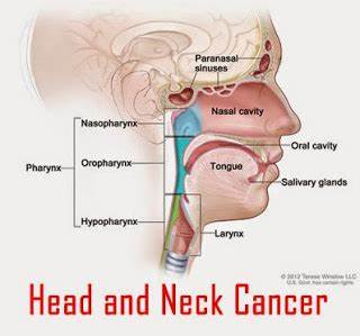
\includegraphics{images/HNC_Kopf.png}
\caption{Most affected tissues and organs by head and neck cancer}
\end{figure}

In the century of next generation sequencing, the genome became an
interesting target for scientists. Approaches that directly affect
important oncogenes often fail due to the fact that these genes play an
important role in healthy cells. The researchers in our paper
(Jerby-Arnon, L., et al. (2014). ``Predicting Cancer-Specific
Vulnerability via Data-Driven Detection of Synthetic Lethality.'' Cell
158(5): 1199-1209.) investigated synthetic lethality and synthetic
dosage lethality that uses gene interactions to affect tumorous
proliferation. Synthetic letahlity describes a gene interaction in which
single-gene defects are compatible with cell viability, but the
combination of gene effects results in cell death. Synthetic dosage
lethality occurs, when the overexpression of one gene is combined with
the knockout of another gene.

\begin{figure}
\centering
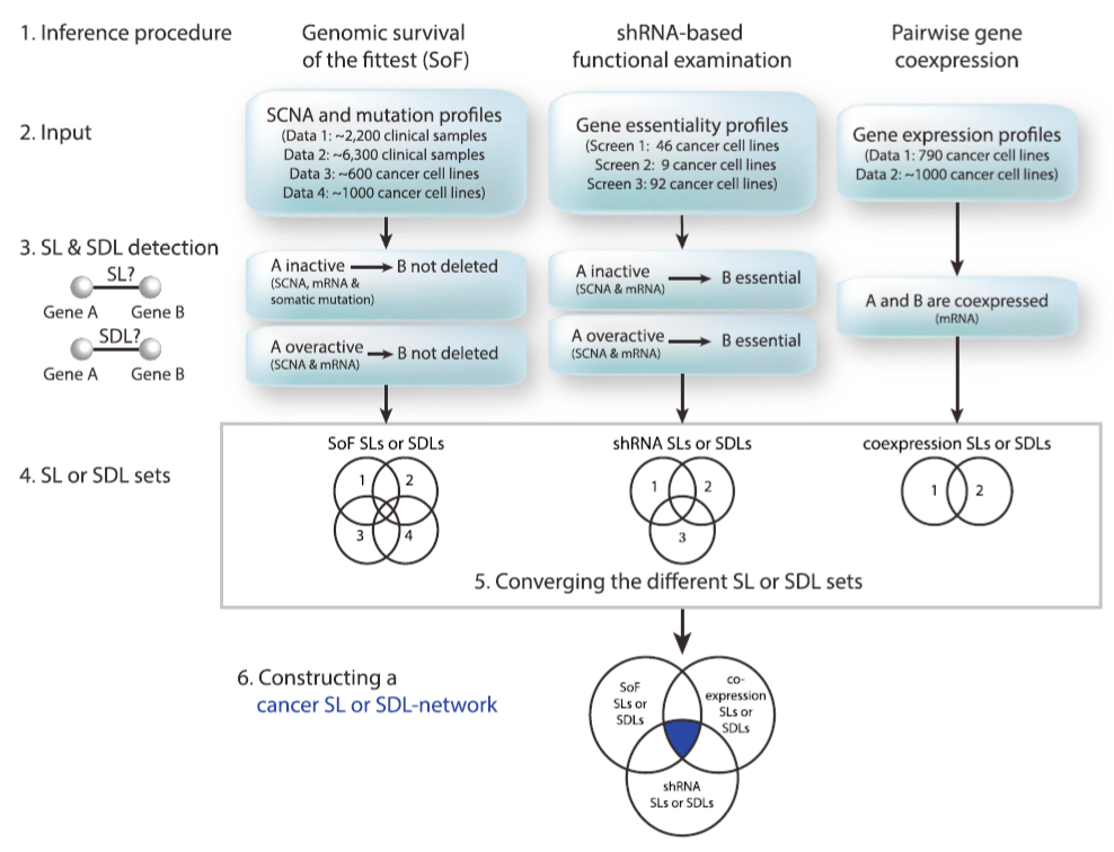
\includegraphics{images/Daisy.png}
\caption{Daisy-System}
\end{figure}

Daisy consists of three statistical approaches (Figure 2), each
processing different sub data from a cancer Dataset. The first strategy
is “Survival of the fittest”, where just deleted SL-paired genes
were selected, that are not in a surviving cancer culture. The second
strategy is “functional examination” where SL genes were identified,
by knocking out genes, with the additive, that the SL partners are
inactive. If the tumor shows decreased proliferation, it accounts for
the SL pair group. The third strategy is “pairwise gene co-
expression” that is based on the fact that SL pairs are often closely
related in biological pathways and therefore exhibit similar occurrence.
If a gene pair fulfills every of the three criteria, it might be a
potential SL pair according to DAISY. To check for SDL partners the
criteria of inactive or active is replaced by under- or overactive,
measured through expression numbers and copy number alterations.

\subsection{Milestones}\label{milestones}

\begin{figure}
\centering
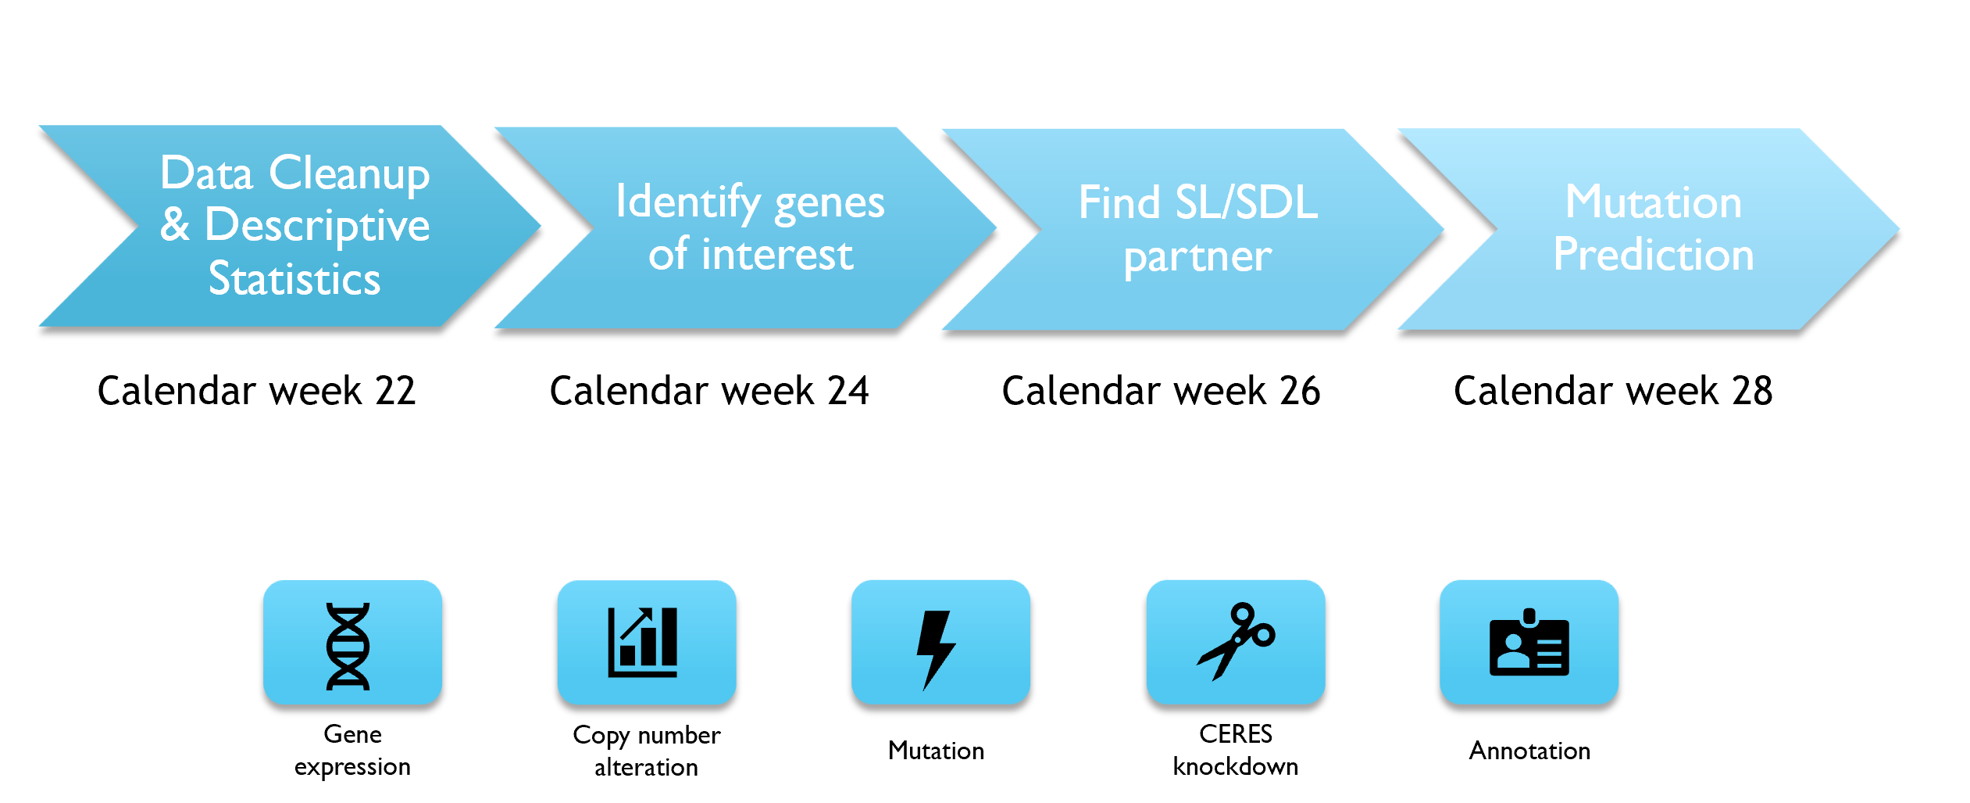
\includegraphics{images/milestones.png}
\caption{Milestones of our project}
\end{figure}

The strategy of our project consisted of 4 main milestones (Figure 3).
At first we familiarized with the data and did the first descriptive
statistics in milestone 1. Secondly, we identified potential genes “of
interest” (SL and SDL candidates), according to DAISY-System. In our
third milestone, the core task of our project was implemented. The
identification of SL and SDL pairs was executed using functional
examination, survival of the fittest and pairwise co-expression. Lastly,
in our fourth milestone we tested logistic regression to predict
mutations.

\section{1. Data Cleanup \& Descriptive
Statistics}\label{data-cleanup-descriptive-statistics}

\subsection{Loading data and defining HNC
variables}\label{loading-data-and-defining-hnc-variables}

\begin{Shaded}
\begin{Highlighting}[]
\CommentTok{# Load dataset}
\NormalTok{allDepMapData =}\StringTok{ }\KeywordTok{readRDS}\NormalTok{(}\StringTok{"DepMap19Q1_allData.RDS"}\NormalTok{)}

\CommentTok{# Creation of sub matrices}
\NormalTok{expression =}\StringTok{ }\NormalTok{allDepMapData[[}\StringTok{"expression"}\NormalTok{]]}
\NormalTok{copynumber =}\StringTok{ }\NormalTok{allDepMapData[[}\StringTok{"copynumber"}\NormalTok{]]}
\NormalTok{mutation =}\StringTok{ }\NormalTok{allDepMapData[[}\StringTok{"mutation"}\NormalTok{]]}
\NormalTok{kd.ceres =}\StringTok{ }\NormalTok{allDepMapData[[}\StringTok{"kd.ceres"}\NormalTok{]]}
\NormalTok{kd.prob =}\StringTok{ }\NormalTok{allDepMapData[[}\StringTok{"kd.prob"}\NormalTok{]]}
\NormalTok{annotation =}\StringTok{ }\NormalTok{allDepMapData[[}\StringTok{"annotation"}\NormalTok{]]}
\KeywordTok{rm}\NormalTok{(allDepMapData)}

\CommentTok{# Reducing the samples to head and neck cancer samples}
\NormalTok{annotation.HNC =}\StringTok{ }\NormalTok{annotation[}\KeywordTok{which}\NormalTok{(annotation}\OperatorTok{$}\NormalTok{Primary.Disease }\OperatorTok{==}\StringTok{ "Head and Neck Cancer"}\NormalTok{), ]}
\NormalTok{ID =}\StringTok{ }\NormalTok{annotation.HNC}\OperatorTok{$}\NormalTok{DepMap_ID}

\CommentTok{# Filtering of sub matrices by primary disease "Head and neck cancer"}
\NormalTok{expression.HNC =}\StringTok{ }\NormalTok{expression[ , }\KeywordTok{which}\NormalTok{(}\KeywordTok{colnames}\NormalTok{(expression) }\OperatorTok\StringTok{ }\NormalTok{ID)]}
\NormalTok{copynumber.HNC =}\StringTok{ }\NormalTok{copynumber[ , }\KeywordTok{which}\NormalTok{(}\KeywordTok{colnames}\NormalTok{(copynumber) }\OperatorTok\StringTok{ }\NormalTok{ID)]}
\NormalTok{kd.ceres.HNC =}\StringTok{ }\NormalTok{kd.ceres[ , }\KeywordTok{which}\NormalTok{(}\KeywordTok{colnames}\NormalTok{(kd.ceres) }\OperatorTok\StringTok{ }\NormalTok{ID)]}
\NormalTok{kd.prob.HNC =}\StringTok{ }\NormalTok{kd.prob[ , }\KeywordTok{which}\NormalTok{(}\KeywordTok{colnames}\NormalTok{(kd.prob) }\OperatorTok\StringTok{ }\NormalTok{ID)]}
\NormalTok{mutation.HNC =}\StringTok{ }\NormalTok{mutation[ID]}
\end{Highlighting}
\end{Shaded}

\subsection{Expression analysis}\label{expression-analysis}

\subsubsection{Checking for NAs}\label{checking-for-nas}

\begin{Shaded}
\begin{Highlighting}[]
\KeywordTok{sum}\NormalTok{(}\KeywordTok{is.na}\NormalTok{(expression) }\OperatorTok{==}\StringTok{ }\OtherTok{TRUE}\NormalTok{)}
\end{Highlighting}
\end{Shaded}

\begin{verbatim}
[1] 0
\end{verbatim}

Result: There are no NAs in the expression data.

\subsubsection{Examine expression
values}\label{examine-expression-values}

Create a reference group of expression data

\begin{Shaded}
\begin{Highlighting}[]
\StringTok{'%!in%'}\NormalTok{ =}\StringTok{ }\ControlFlowTok{function}\NormalTok{(x,y)}\OperatorTok{!}\NormalTok{(}\StringTok{'%in%'}\NormalTok{(x,y)) }\CommentTok{# Define function "is not in"}

\NormalTok{expression.reference =}\StringTok{ }\NormalTok{expression[ , }\KeywordTok{which}\NormalTok{(}\KeywordTok{colnames}\NormalTok{(expression) }\OperatorTok\StringTok{ }\NormalTok{ID)]}
\end{Highlighting}
\end{Shaded}

and calculate their mean.

\begin{Shaded}
\begin{Highlighting}[]
\NormalTok{mean.exp.reference =}\StringTok{ }\KeywordTok{apply}\NormalTok{(expression.reference, }\DecValTok{1}\NormalTok{, mean)}
\NormalTok{mean.exp.HNC =}\StringTok{ }\KeywordTok{apply}\NormalTok{(expression.HNC, }\DecValTok{1}\NormalTok{, mean)}
\end{Highlighting}
\end{Shaded}

Firstly, we want to check if the gene expressions of the HNC samples and
the reference group are normally distributed.

\begin{Shaded}
\begin{Highlighting}[]
\NormalTok{HNC =}\StringTok{ }\KeywordTok{data.frame}\NormalTok{(}\DataTypeTok{expression_values =}\NormalTok{ mean.exp.HNC, }\DataTypeTok{sample =} \StringTok{"HNC"}\NormalTok{)}
\NormalTok{Reference =}\StringTok{ }\KeywordTok{data.frame}\NormalTok{(}\DataTypeTok{expression_values =}\NormalTok{ mean.exp.reference, }\DataTypeTok{sample =} \StringTok{"Reference"}\NormalTok{)}
\NormalTok{mean.expression =}\StringTok{ }\KeywordTok{rbind}\NormalTok{(Reference, HNC)}

\KeywordTok{ggqqplot}\NormalTok{(mean.expression, }\DataTypeTok{x =} \StringTok{"expression_values"}\NormalTok{,}
   \DataTypeTok{color =} \StringTok{"sample"}\NormalTok{,}
   \DataTypeTok{palette =} \KeywordTok{c}\NormalTok{(}\StringTok{"#FC4E07"}\NormalTok{, }\StringTok{"#0073C2FF"}\NormalTok{), }\CommentTok{# Red and blue}
   \DataTypeTok{ggtheme =} \KeywordTok{theme_pubclean}\NormalTok{())}
\end{Highlighting}
\end{Shaded}

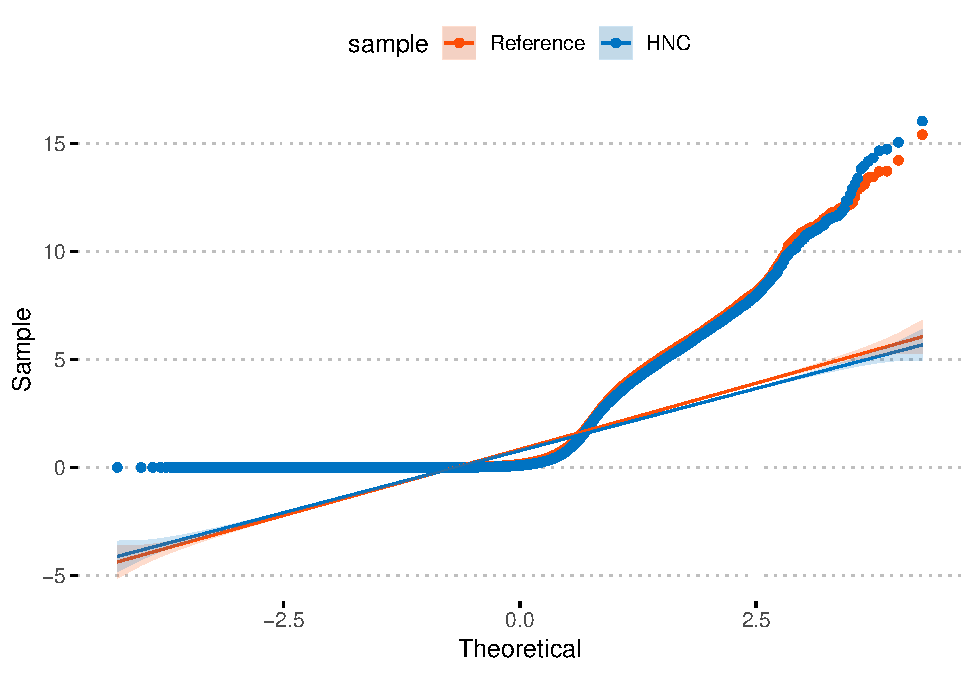
\includegraphics{Project_HNC_files/figure-latex/1_expression_values3-1.pdf}

Result: Gene espression is neither in HNC samples nor in reference
samples normally distributed.

Then we compare HNC and reference group gene expression using a
statistical test. A Wilcoxon rank sum test must be applied because the
expression is not normally distributed.

\begin{Shaded}
\begin{Highlighting}[]
\KeywordTok{wilcox.test}\NormalTok{(mean.exp.HNC, mean.exp.reference)}
\end{Highlighting}
\end{Shaded}

\begin{verbatim}

    Wilcoxon rank sum test with continuity correction

data:  mean.exp.HNC and mean.exp.reference
W = 1080700000, p-value < 2.2e-16
alternative hypothesis: true location shift is not equal to 0
\end{verbatim}

Result: Mean gene expression differs between HNC and reference group
samples significantly.

Next we check if the gene expression differs whether a gene has a
deleterious mutation or not. AS an example, we compare the mean TP53
gene expression of all samples with and without deleterious TP53
mutation.

\begin{Shaded}
\begin{Highlighting}[]
\CommentTok{# Get the ID of samples whith and without deleterious mutation}
\NormalTok{TP53.mut.ID =}\StringTok{ }\KeywordTok{lapply}\NormalTok{(}\DecValTok{1}\OperatorTok{:}\KeywordTok{length}\NormalTok{(mutation), }\ControlFlowTok{function}\NormalTok{(a) \{}
\NormalTok{  dat_picker =}\StringTok{ }\NormalTok{mutation[[a]]}
\NormalTok{  dat_picker =}\StringTok{ }\NormalTok{dat_picker[}\KeywordTok{which}\NormalTok{(dat_picker}\OperatorTok{$}\NormalTok{isDeleterious }\OperatorTok{==}\StringTok{ }\OtherTok{TRUE}\NormalTok{),]}
\NormalTok{  out =}\StringTok{ }\KeywordTok{ifelse}\NormalTok{(}\StringTok{"TP53"} \OperatorTok\StringTok{ }\NormalTok{dat_picker}\OperatorTok{$}\NormalTok{Hugo_Symbol, a, }\OtherTok{NA}\NormalTok{) }\CommentTok{# Filter all IDs which have a deleterious mutation of TP53}
    \KeywordTok{return}\NormalTok{(out)}
\NormalTok{  \})}

\NormalTok{TP53.not_mut.ID =}\StringTok{ }\KeywordTok{grep}\NormalTok{(}\StringTok{"NA"}\NormalTok{, TP53.mut.ID) }\CommentTok{# ID of samples with no TP53 mutation}
\NormalTok{TP53.mut.ID =}\StringTok{ }\KeywordTok{as.integer}\NormalTok{(TP53.mut.ID[}\KeywordTok{is.na}\NormalTok{(TP53.mut.ID) }\OperatorTok{==}\StringTok{ }\OtherTok{FALSE}\NormalTok{]) }\CommentTok{# ID of samples with TP53 mutation}

\CommentTok{# Create two vectors of expression values}
\NormalTok{exp.TP53.mut =}\StringTok{ }\KeywordTok{as.numeric}\NormalTok{(expression[}\StringTok{"TP53"}\NormalTok{, TP53.mut.ID]) }\CommentTok{# Expression of TP53 deleterious mutated samples}
\NormalTok{exp.TP53.not_mut =}\StringTok{ }\KeywordTok{as.numeric}\NormalTok{(expression[}\StringTok{"TP53"}\NormalTok{, TP53.not_mut.ID]) }\CommentTok{# Expression of TP53 not deleterious mutated samples}
\end{Highlighting}
\end{Shaded}

Compare the expression values by applying Wilcoxon rank sum test.

\begin{Shaded}
\begin{Highlighting}[]
\KeywordTok{wilcox.test}\NormalTok{(exp.TP53.mut , exp.TP53.not_mut)}
\end{Highlighting}
\end{Shaded}

\begin{verbatim}

    Wilcoxon rank sum test with continuity correction

data:  exp.TP53.mut and exp.TP53.not_mut
W = 8276.5, p-value < 2.2e-16
alternative hypothesis: true location shift is not equal to 0
\end{verbatim}

Result: Gene expression of TP53 as an example gene varies significantly
whether the samples has or has no deleterious TP53 mutation.

At last, we plot a histogram to check how the expression values are
distributed.

\begin{Shaded}
\begin{Highlighting}[]
\KeywordTok{gghistogram}\NormalTok{(}\KeywordTok{as.data.frame}\NormalTok{(mean.exp.HNC),}
            \DataTypeTok{x =} \StringTok{"mean.exp.HNC"}\NormalTok{,}
            \DataTypeTok{xlab =} \StringTok{"expression value"}\NormalTok{,}
            \DataTypeTok{bins =} \DecValTok{60}\NormalTok{,}
            \DataTypeTok{fill =} \StringTok{"#0073C2FF"}\NormalTok{,}
            \DataTypeTok{color =} \StringTok{"#0073C2FF"}\NormalTok{,}
            \DataTypeTok{add =} \StringTok{"mean"}\NormalTok{,}
            \DataTypeTok{rug =} \OtherTok{TRUE}\NormalTok{)}
\end{Highlighting}
\end{Shaded}

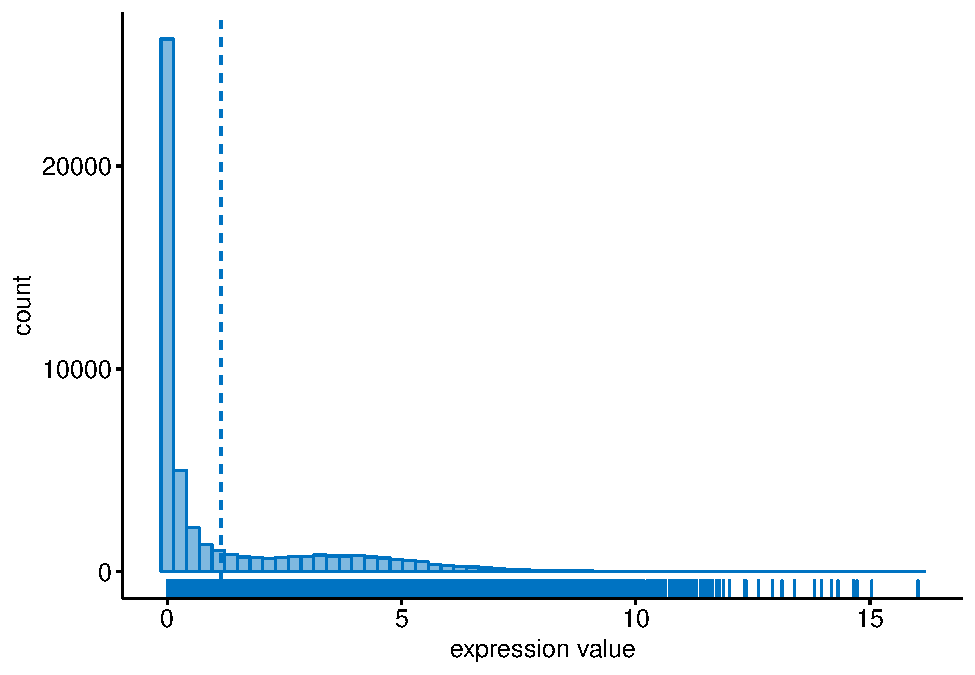
\includegraphics{Project_HNC_files/figure-latex/1_expression_values7-1.pdf}

Result: The most genes have expression values around 0.

\subsubsection{Plot the 20 most under- and overexpressed genes of HNC
samples.}\label{plot-the-20-most-under--and-overexpressed-genes-of-hnc-samples.}

For this we need to normalize the expression data from HNC samples

\begin{Shaded}
\begin{Highlighting}[]
\NormalTok{expr.HNC.norm =}\StringTok{ }\KeywordTok{as.data.frame}\NormalTok{(}\KeywordTok{apply}\NormalTok{(expression.HNC, }\DecValTok{2}\NormalTok{, }\ControlFlowTok{function}\NormalTok{(x) \{}
\NormalTok{  x }\OperatorTok{-}\StringTok{ }\NormalTok{mean.exp.reference}
\NormalTok{\}))}
\end{Highlighting}
\end{Shaded}

and calculate the mean of the normalesid expression values.

\begin{Shaded}
\begin{Highlighting}[]
\NormalTok{mean.expr.HNC.norm =}\StringTok{ }\KeywordTok{as.data.frame}\NormalTok{(}\KeywordTok{apply}\NormalTok{(expr.HNC.norm, }\DecValTok{1}\NormalTok{, mean))}
\end{Highlighting}
\end{Shaded}

Then create a dataframe with needed information for the barplot

\begin{Shaded}
\begin{Highlighting}[]
\NormalTok{barplot.data =}\StringTok{ }\KeywordTok{data.frame}\NormalTok{(}\DataTypeTok{Genes=}\KeywordTok{rownames}\NormalTok{(expr.HNC.norm),}
                          \DataTypeTok{Values=}\NormalTok{mean.expr.HNC.norm)}
\KeywordTok{names}\NormalTok{(barplot.data) =}\StringTok{ }\KeywordTok{c}\NormalTok{(}\StringTok{"Genes"}\NormalTok{, }\StringTok{"Values"}\NormalTok{)}
\NormalTok{barplot.data}\OperatorTok{$}\NormalTok{Group =}\StringTok{ }\KeywordTok{ifelse}\NormalTok{(barplot.data}\OperatorTok{$}\NormalTok{Values}\OperatorTok{>}\DecValTok{0}\NormalTok{,}\StringTok{"overexpressed"}\NormalTok{,}\StringTok{"underexpressed"}\NormalTok{)}
\NormalTok{barplot.data =}\StringTok{ }\NormalTok{barplot.data[}\KeywordTok{order}\NormalTok{(barplot.data}\OperatorTok{$}\NormalTok{Values),]}
\NormalTok{barplot.data =}\StringTok{ }\NormalTok{barplot.data[}\KeywordTok{c}\NormalTok{(}\DecValTok{1}\OperatorTok{:}\DecValTok{19}\NormalTok{, (}\KeywordTok{nrow}\NormalTok{(barplot.data)}\OperatorTok{-}\DecValTok{20}\NormalTok{)}\OperatorTok{:}\KeywordTok{nrow}\NormalTok{(barplot.data)),]}
\end{Highlighting}
\end{Shaded}

and plot this dataframe.

\begin{Shaded}
\begin{Highlighting}[]
\KeywordTok{ggplot}\NormalTok{(barplot.data,}\KeywordTok{aes}\NormalTok{(}\DataTypeTok{x=}\NormalTok{Genes,}\DataTypeTok{y=}\NormalTok{Values,}\DataTypeTok{fill=}\NormalTok{Group)) }\OperatorTok{+}
\StringTok{  }\KeywordTok{ylab}\NormalTok{(}\StringTok{"Normalized mean expression values"}\NormalTok{) }\OperatorTok{+}
\StringTok{  }\KeywordTok{geom_bar}\NormalTok{(}\DataTypeTok{stat=}\StringTok{"identity"}\NormalTok{) }\OperatorTok{+}
\StringTok{  }\KeywordTok{coord_flip}\NormalTok{() }\OperatorTok{+}
\StringTok{  }\KeywordTok{theme}\NormalTok{(}\DataTypeTok{axis.text.y =} \KeywordTok{element_text}\NormalTok{(}\DataTypeTok{size=}\DecValTok{6}\NormalTok{))}
\end{Highlighting}
\end{Shaded}

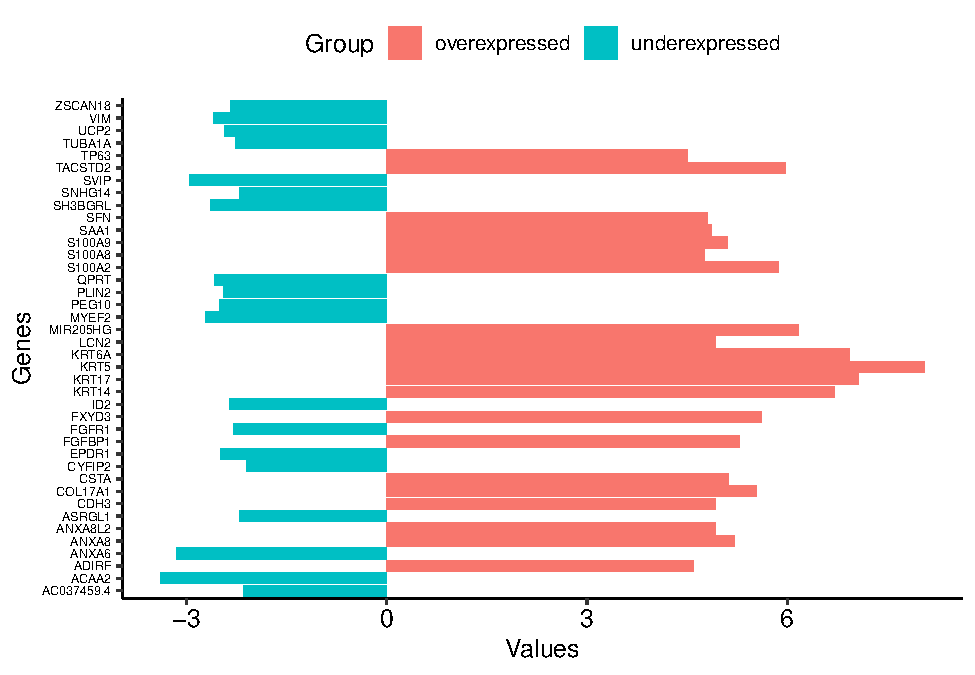
\includegraphics{Project_HNC_files/figure-latex/1_expression_plot4-1.pdf}

\subsubsection{Cleanup of the
enviroment}\label{cleanup-of-the-enviroment}

\begin{Shaded}
\begin{Highlighting}[]
\KeywordTok{rm}\NormalTok{(HNC, Reference, mean.expression, TP53.mut.ID, TP53.not_mut.ID, exp.TP53.mut, exp.TP53.not_mut, mean.expr.HNC.norm, barplot.data, mean.exp.HNC, mean.exp.reference, expression.reference)}
\end{Highlighting}
\end{Shaded}

\subsection{Copynumber Alteration}\label{copynumber-alteration}

\subsubsection{Analysis of NA values}\label{analysis-of-na-values}

Examination of NA values in the copynumber.HNC data

\begin{Shaded}
\begin{Highlighting}[]
\CommentTok{# Sum up all NAs in each row}
\NormalTok{NA.rows =}\StringTok{ }\KeywordTok{apply}\NormalTok{(copynumber.HNC,}\DecValTok{1}\NormalTok{, }\ControlFlowTok{function}\NormalTok{(x) \{}
          \KeywordTok{sum}\NormalTok{(}\KeywordTok{is.na}\NormalTok{(x))}
\NormalTok{\})}
\CommentTok{# Define all rows cotaining missing values}
\NormalTok{NA.rows =}\StringTok{ }\KeywordTok{which}\NormalTok{( NA.rows }\OperatorTok{>}\StringTok{ }\DecValTok{0}\NormalTok{)}
\KeywordTok{length}\NormalTok{(NA.rows)}
\end{Highlighting}
\end{Shaded}

\begin{verbatim}
[1] 107
\end{verbatim}

Only 107 out of 23299 gens have NA values and are therefore deleted from
the copynumber.HNC dataframe

\begin{Shaded}
\begin{Highlighting}[]
\NormalTok{copynumber.HNC =}\StringTok{ }\NormalTok{copynumber.HNC[}\OperatorTok{-}\NormalTok{NA.rows,]}
\KeywordTok{dim}\NormalTok{(copynumber.HNC)}
\end{Highlighting}
\end{Shaded}

\begin{verbatim}
[1] 23192    27
\end{verbatim}

Creating a reference data and examination of its NA values

\begin{Shaded}
\begin{Highlighting}[]
\NormalTok{copynumber.reference =}\StringTok{ }\NormalTok{copynumber[,}\KeywordTok{which}\NormalTok{(}\KeywordTok{colnames}\NormalTok{(copynumber) }\OperatorTok\StringTok{ }\NormalTok{ID)]}
\KeywordTok{dim}\NormalTok{(copynumber.reference)}
\end{Highlighting}
\end{Shaded}

\begin{verbatim}
[1] 23299   517
\end{verbatim}

\begin{Shaded}
\begin{Highlighting}[]
\NormalTok{NA.rows.ref =}\StringTok{ }\KeywordTok{apply}\NormalTok{(copynumber.reference,}\DecValTok{1}\NormalTok{, }\ControlFlowTok{function}\NormalTok{(x) \{}
          \KeywordTok{sum}\NormalTok{(}\KeywordTok{is.na}\NormalTok{(x))}
\NormalTok{\})}
\NormalTok{NA.rows.ref =}\StringTok{ }\KeywordTok{which}\NormalTok{( NA.rows.ref }\OperatorTok{>}\StringTok{ }\DecValTok{0}\NormalTok{)}
\KeywordTok{length}\NormalTok{(NA.rows.ref)}
\end{Highlighting}
\end{Shaded}

\begin{verbatim}
[1] 107
\end{verbatim}

\begin{Shaded}
\begin{Highlighting}[]
\KeywordTok{summary}\NormalTok{(NA.rows }\OperatorTok{==}\StringTok{ }\NormalTok{NA.rows.ref)}
\end{Highlighting}
\end{Shaded}

\begin{verbatim}
   Mode    TRUE 
logical     107 
\end{verbatim}

Genes with NA values are the same for the HNC samples and all the other
samples. Therefore, they can be deleted in the reference data as well.

\begin{Shaded}
\begin{Highlighting}[]
\NormalTok{copynumber.reference =}\StringTok{ }\NormalTok{copynumber.reference[}\OperatorTok{-}\NormalTok{NA.rows.ref,]}
\NormalTok{copynumber =}\StringTok{ }\NormalTok{copynumber[}\OperatorTok{-}\NormalTok{NA.rows.ref,]}
\KeywordTok{dim}\NormalTok{(copynumber.reference)}
\end{Highlighting}
\end{Shaded}

\begin{verbatim}
[1] 23192   517
\end{verbatim}

\begin{Shaded}
\begin{Highlighting}[]
\KeywordTok{dim}\NormalTok{(copynumber)}
\end{Highlighting}
\end{Shaded}

\begin{verbatim}
[1] 23192   544
\end{verbatim}

\subsubsection{Normalisation of the copynumber
values}\label{normalisation-of-the-copynumber-values}

For the HNC normalisation we will use the mean CN value per gen of the
reference data.

\begin{Shaded}
\begin{Highlighting}[]
\NormalTok{copynumber.ref.mean =}\StringTok{ }\KeywordTok{apply}\NormalTok{(copynumber.reference,}\DecValTok{1}\NormalTok{, mean)}
\NormalTok{copynumber.HNC.mean =}\StringTok{ }\KeywordTok{apply}\NormalTok{(copynumber.HNC ,}\DecValTok{1}\NormalTok{, mean)}
\end{Highlighting}
\end{Shaded}

Creating a dataframe of all copynumber values. The values are normalized
to the mean copynumbers of the reference data.

\begin{Shaded}
\begin{Highlighting}[]
\NormalTok{cna.HNC.norm =}\StringTok{ }\KeywordTok{as.data.frame}\NormalTok{(}\KeywordTok{apply}\NormalTok{(copynumber.HNC, }\DecValTok{2}\NormalTok{, }\ControlFlowTok{function}\NormalTok{(x) \{}
\NormalTok{  x }\OperatorTok{-}\StringTok{ }\NormalTok{copynumber.ref.mean}
\NormalTok{\}))}
\end{Highlighting}
\end{Shaded}

Creating a dataframe of HNC copynumber values. The values are normalized
to the mean copynumbers of the reference data. For further analysing the
dataframe is ordered in a decreasing manner.

\begin{Shaded}
\begin{Highlighting}[]
\NormalTok{Values =}\StringTok{ }\NormalTok{copynumber.HNC.mean }\OperatorTok{-}\StringTok{ }\NormalTok{copynumber.ref.mean}
\NormalTok{copynumber.HNC.norm =}\StringTok{ }\KeywordTok{data.frame}\NormalTok{(}\DataTypeTok{values =} \KeywordTok{sort}\NormalTok{(Values, }\DataTypeTok{decreasing =} \OtherTok{TRUE}\NormalTok{), }\DataTypeTok{genes =} \KeywordTok{row.names}\NormalTok{(copynumber.HNC))}
\NormalTok{copynumber.HNC.norm}\OperatorTok{$}\NormalTok{Group =}\StringTok{ }\KeywordTok{ifelse}\NormalTok{(copynumber.HNC.norm}\OperatorTok{$}\NormalTok{values }\OperatorTok{>}\StringTok{ }\DecValTok{0}\NormalTok{,}\StringTok{"high CN"}\NormalTok{,}\StringTok{"low CN"}\NormalTok{)}
\end{Highlighting}
\end{Shaded}

Plotting genes with the highest and lowest copynumbers.

\begin{Shaded}
\begin{Highlighting}[]
\KeywordTok{ggplot}\NormalTok{(copynumber.HNC.norm[}\KeywordTok{c}\NormalTok{(}\DecValTok{1}\OperatorTok{:}\DecValTok{20}\NormalTok{,}\DecValTok{23172}\OperatorTok{:}\DecValTok{23192}\NormalTok{),],}\KeywordTok{aes}\NormalTok{(}\DataTypeTok{x=}\NormalTok{genes,}\DataTypeTok{y=}\NormalTok{values,}\DataTypeTok{fill=}\NormalTok{Group)) }\OperatorTok{+}
\StringTok{  }\KeywordTok{geom_bar}\NormalTok{(}\DataTypeTok{stat=}\StringTok{"identity"}\NormalTok{) }\OperatorTok{+}
\StringTok{  }\KeywordTok{ylab}\NormalTok{(}\StringTok{"Normalized mean CNA values"}\NormalTok{) }\OperatorTok{+}
\StringTok{  }\KeywordTok{coord_flip}\NormalTok{() }\OperatorTok{+}
\StringTok{  }\KeywordTok{theme}\NormalTok{(}\DataTypeTok{axis.text.y =} \KeywordTok{element_text}\NormalTok{(}\DataTypeTok{size=}\DecValTok{6}\NormalTok{))}
\end{Highlighting}
\end{Shaded}

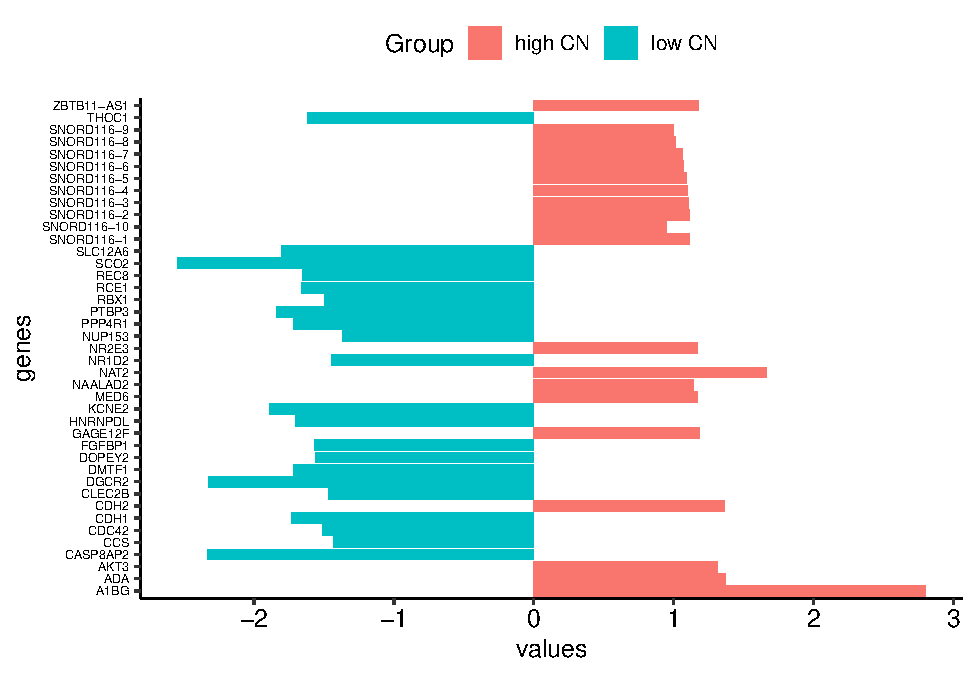
\includegraphics{Project_HNC_files/figure-latex/1_copynumber_plot-1.pdf}

\subsubsection{Cleanup of the
environment}\label{cleanup-of-the-environment}

\begin{Shaded}
\begin{Highlighting}[]
\KeywordTok{rm}\NormalTok{(NA.rows, NA.rows.ref, copynumber.HNC.norm, copynumber.HNC.mean, copynumber.ref.mean, copynumber.reference, Values)}
\end{Highlighting}
\end{Shaded}

\subsection{Mutation}\label{mutation}

\subsubsection{Find Mutations with the highest
frequencies}\label{find-mutations-with-the-highest-frequencies}

Melt all mutation matrices together as data frame and find out most
frequent mutations

\begin{Shaded}
\begin{Highlighting}[]
\NormalTok{all_mutations =}\StringTok{ }\KeywordTok{do.call}\NormalTok{(rbind,mutation)}
\NormalTok{all_mutated_genes =}\StringTok{ }\KeywordTok{table}\NormalTok{(all_mutations}\OperatorTok{$}\NormalTok{Hugo_Symbol)}
\NormalTok{all_mutated_genes_df =}\StringTok{ }\KeywordTok{as.data.frame}\NormalTok{(all_mutated_genes)}
\end{Highlighting}
\end{Shaded}

Order the found mutations by frequencies and extract 30 most frequent

\begin{Shaded}
\begin{Highlighting}[]
\NormalTok{ID_all_highest_frequencies =}\StringTok{ }\KeywordTok{head}\NormalTok{(}\KeywordTok{order}\NormalTok{(all_mutated_genes_df[[}\StringTok{"Freq"}\NormalTok{]], }\DataTypeTok{decreasing =} \OtherTok{TRUE}\NormalTok{), }\DecValTok{30}\NormalTok{)}
\NormalTok{all_mutated_genes_df_highest_}\DecValTok{30}\NormalTok{ =}\StringTok{ }\NormalTok{all_mutated_genes_df[}\KeywordTok{which}\NormalTok{(}\KeywordTok{rownames}\NormalTok{(all_mutated_genes_df) }\OperatorTok\StringTok{ }\NormalTok{ID_all_highest_frequencies), ]}
\NormalTok{ID_all_highest_30_frequencies =}\StringTok{ }\KeywordTok{order}\NormalTok{(all_mutated_genes_df_highest_}\DecValTok{30}\NormalTok{[}\StringTok{"Freq"}\NormalTok{], }\DataTypeTok{decreasing =} \OtherTok{TRUE}\NormalTok{) }
\NormalTok{all_mutated_genes_highest_30_ordered =}\StringTok{ }\NormalTok{all_mutated_genes_df_highest_}\DecValTok{30}\NormalTok{[ID_all_highest_30_frequencies, ]}
\KeywordTok{head}\NormalTok{(all_mutated_genes_highest_30_ordered)}
\end{Highlighting}
\end{Shaded}

\begin{verbatim}
        Var1 Freq
17577    TTN 1567
10296  MUC16  774
17193   TP53  471
10213 MT-ND5  439
11210  OBSCN  368
10304   MUC4  361
\end{verbatim}

Name the newly established data frame for the look

\begin{Shaded}
\begin{Highlighting}[]
\NormalTok{ID_all_highest_30_frequencies =}\StringTok{ }\KeywordTok{order}\NormalTok{(all_mutated_genes_df_highest_}\DecValTok{30}\NormalTok{[}\StringTok{"Freq"}\NormalTok{], }\DataTypeTok{decreasing =} \OtherTok{TRUE}\NormalTok{)}
\NormalTok{all_mutated_genes_df_highest_30_ordered =}\StringTok{ }\NormalTok{all_mutated_genes_df_highest_}\DecValTok{30}\NormalTok{[ID_all_highest_30_frequencies, ]}
\KeywordTok{rownames}\NormalTok{(all_mutated_genes_df_highest_30_ordered) =}\StringTok{ }\DecValTok{1}\OperatorTok{:}\DecValTok{30}
\NormalTok{colnames_ordered =}\StringTok{ }\KeywordTok{c}\NormalTok{(}\StringTok{"Gene"}\NormalTok{, }\StringTok{"Freq"}\NormalTok{)}
\KeywordTok{colnames}\NormalTok{(all_mutated_genes_df_highest_30_ordered) =}\StringTok{ }\NormalTok{colnames_ordered}
\end{Highlighting}
\end{Shaded}

Melt only HNC sample mutation matrices together and find out most
frequent mutations

\begin{Shaded}
\begin{Highlighting}[]
\NormalTok{HNC_mutations =}\StringTok{ }\KeywordTok{do.call}\NormalTok{(rbind, mutation.HNC)}
\NormalTok{HNC_mutated_genes =}\StringTok{ }\KeywordTok{table}\NormalTok{(HNC_mutations}\OperatorTok{$}\NormalTok{Hugo_Symbol)}
\NormalTok{HNC_mutated_genes_df =}\StringTok{ }\KeywordTok{as.data.frame}\NormalTok{(HNC_mutated_genes)}
\end{Highlighting}
\end{Shaded}

Order the found mutations by frequencies and name the data frame

\begin{Shaded}
\begin{Highlighting}[]
\NormalTok{ID_HNC_highest_frequencies =}\StringTok{ }\KeywordTok{head}\NormalTok{(}\KeywordTok{order}\NormalTok{(HNC_mutated_genes_df[[}\StringTok{"Freq"}\NormalTok{]], }\DataTypeTok{decreasing =} \OtherTok{TRUE}\NormalTok{), }\KeywordTok{length}\NormalTok{(ID))}
\NormalTok{HNC_mutated_genes_df_highest_ordered =}\StringTok{ }\NormalTok{HNC_mutated_genes_df[ID_HNC_highest_frequencies, ]}
\KeywordTok{rownames}\NormalTok{(HNC_mutated_genes_df_highest_ordered) =}\StringTok{ }\DecValTok{1}\OperatorTok{:}\KeywordTok{length}\NormalTok{(ID)}
\KeywordTok{colnames}\NormalTok{(HNC_mutated_genes_df_highest_ordered) =}\StringTok{ }\NormalTok{colnames_ordered}
\end{Highlighting}
\end{Shaded}

\subsubsection{Plotting mutation frequencies of all samples and of HNC
samples}\label{plotting-mutation-frequencies-of-all-samples-and-of-hnc-samples}

Plot mutations in all samples

\begin{Shaded}
\begin{Highlighting}[]
\KeywordTok{ggplot}\NormalTok{(}\DataTypeTok{data =}\NormalTok{ all_mutated_genes_df_highest_30_ordered, }\KeywordTok{aes}\NormalTok{(}\DataTypeTok{x=}\NormalTok{Gene, }\DataTypeTok{y=}\NormalTok{Freq)) }\OperatorTok{+}
\StringTok{  }\KeywordTok{geom_bar}\NormalTok{(}\DataTypeTok{stat =} \StringTok{"identity"}\NormalTok{, }\DataTypeTok{width =} \FloatTok{0.5}\NormalTok{, }\DataTypeTok{fill=}\StringTok{"steelblue"}\NormalTok{) }\OperatorTok{+}
\StringTok{  }\KeywordTok{geom_text}\NormalTok{(}\KeywordTok{aes}\NormalTok{(}\DataTypeTok{label=}\NormalTok{Freq), }\DataTypeTok{vjust=}\OperatorTok{-}\FloatTok{0.3}\NormalTok{, }\DataTypeTok{size=}\FloatTok{2.5}\NormalTok{) }\OperatorTok{+}
\StringTok{  }\KeywordTok{theme_grey}\NormalTok{() }\OperatorTok{+}\StringTok{ }\KeywordTok{coord_flip}\NormalTok{()}
\end{Highlighting}
\end{Shaded}

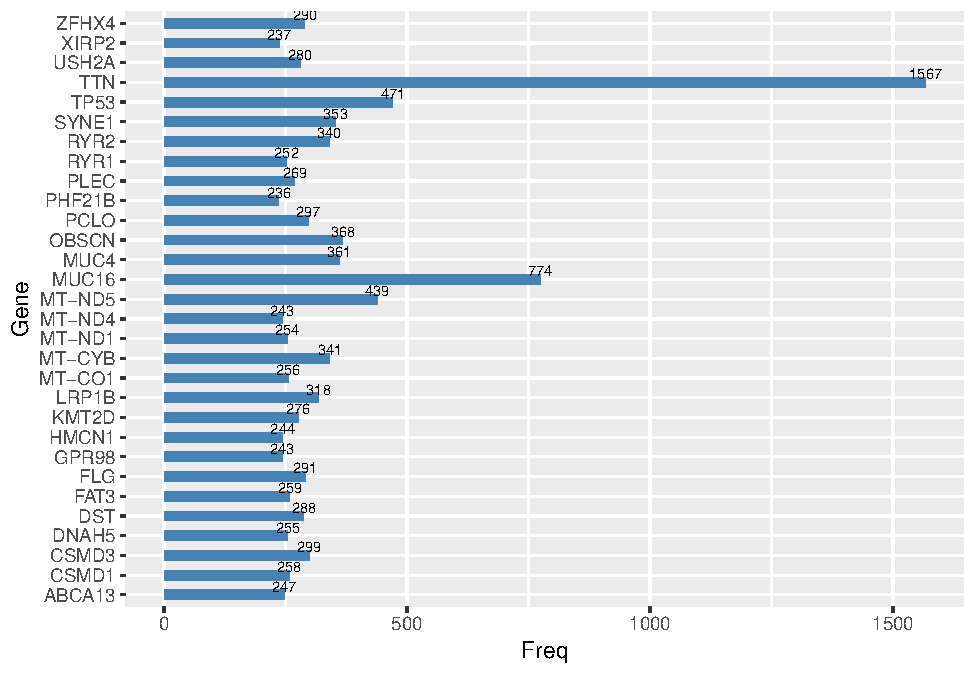
\includegraphics{Project_HNC_files/figure-latex/1_muation_frequency3-1.pdf}

Plot mutations in HNC samples

\begin{Shaded}
\begin{Highlighting}[]
\KeywordTok{ggplot}\NormalTok{(}\DataTypeTok{data =}\NormalTok{ HNC_mutated_genes_df_highest_ordered, }\KeywordTok{aes}\NormalTok{(}\DataTypeTok{x=}\NormalTok{Gene, }\DataTypeTok{y=}\NormalTok{Freq)) }\OperatorTok{+}
\StringTok{  }\KeywordTok{geom_bar}\NormalTok{(}\DataTypeTok{stat =} \StringTok{"identity"}\NormalTok{, }\DataTypeTok{width =} \FloatTok{0.5}\NormalTok{, }\DataTypeTok{fill=}\StringTok{"steelblue"}\NormalTok{) }\OperatorTok{+}
\StringTok{  }\KeywordTok{geom_text}\NormalTok{(}\KeywordTok{aes}\NormalTok{(}\DataTypeTok{label=}\NormalTok{Freq), }\DataTypeTok{vjust=}\OperatorTok{-}\FloatTok{0.3}\NormalTok{, }\DataTypeTok{size=}\FloatTok{3.5}\NormalTok{) }\OperatorTok{+}
\StringTok{  }\KeywordTok{theme_grey}\NormalTok{() }\OperatorTok{+}
\StringTok{  }\KeywordTok{coord_flip}\NormalTok{()}
\end{Highlighting}
\end{Shaded}

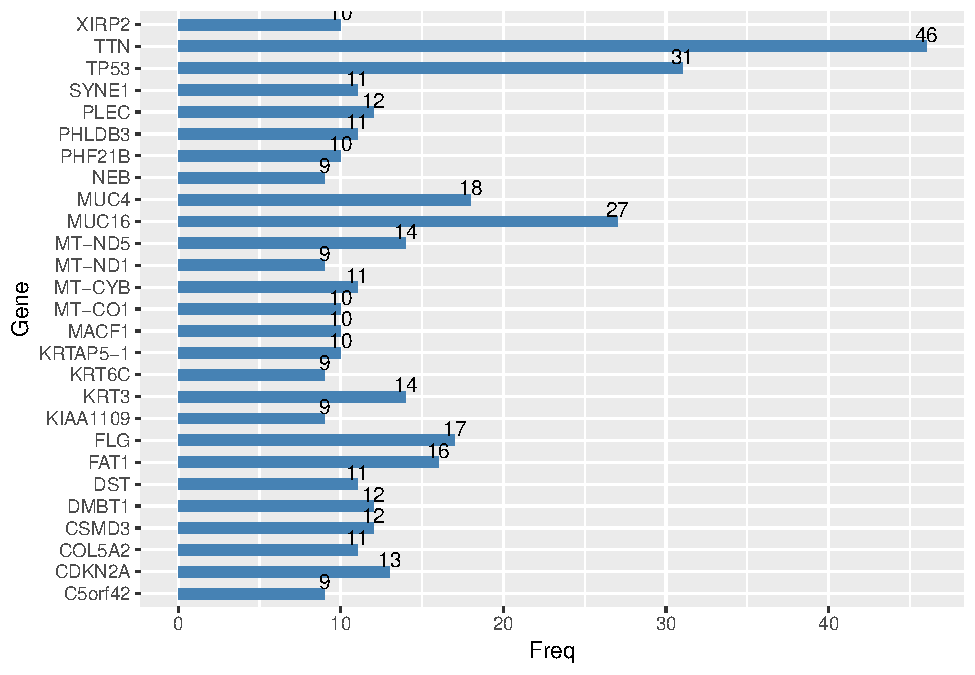
\includegraphics{Project_HNC_files/figure-latex/1_muation_frequency4-1.pdf}

\subsubsection{Clean mutation from unnecessary
data}\label{clean-mutation-from-unnecessary-data}

Due to the needed conditions in the following ``Daisy-tests'' we now
clean the mutation data and extract all ``isDeleterious'' mutations,
since they are essential for the survival or death of a cell. In this
way, we later are able to find our genes of interest for the SL more
easily.

\begin{Shaded}
\begin{Highlighting}[]
\CommentTok{# Generating a function that searches all elements a of our mutation data set which are isDeleterious}
\StringTok{'mutation.clean'}\NormalTok{ =}\StringTok{ }\ControlFlowTok{function}\NormalTok{(data)\{}
\NormalTok{  cleaned_data =}\StringTok{ }\KeywordTok{lapply}\NormalTok{(}\DecValTok{1}\OperatorTok{:}\KeywordTok{length}\NormalTok{(data), }\ControlFlowTok{function}\NormalTok{(a) \{ }\CommentTok{# Data will be mutation (length of 544) or mutation.HNC (length of 27)}
\NormalTok{    dat_picker =}\StringTok{ }\NormalTok{data[[a]] }\CommentTok{# Pick the element of the list on position 'a'}
\NormalTok{    dat_picker =}\StringTok{ }\NormalTok{dat_picker[, }\KeywordTok{c}\NormalTok{(}\StringTok{"Hugo_Symbol"}\NormalTok{, }\StringTok{"isDeleterious"}\NormalTok{)] }\CommentTok{# Choose only the columns with gene name and whether they have a deleterious mutation}
\NormalTok{    dat_picker =}\StringTok{ }\NormalTok{dat_picker[}\KeywordTok{which}\NormalTok{(dat_picker}\OperatorTok{$}\NormalTok{isDeleterious }\OperatorTok{==}\StringTok{ }\OtherTok{TRUE}\NormalTok{),] }\CommentTok{# Choose only deleterious mutations}
    \KeywordTok{return}\NormalTok{(dat_picker)}
\NormalTok{  \})}
  \KeywordTok{names}\NormalTok{(cleaned_data) =}\StringTok{ }\KeywordTok{names}\NormalTok{(data) }\CommentTok{# Keep the names of the input data}
  \KeywordTok{return}\NormalTok{(cleaned_data)}
\NormalTok{\}}
\CommentTok{# Apply the new function on our two mutation data sets in order to clean them}
\NormalTok{mutation =}\StringTok{ }\KeywordTok{mutation.clean}\NormalTok{(mutation)}
\NormalTok{mutation.HNC =}\StringTok{ }\KeywordTok{mutation.clean}\NormalTok{(mutation.HNC)}
\KeywordTok{head}\NormalTok{(mutation.HNC[[}\DecValTok{1}\NormalTok{]])}
\end{Highlighting}
\end{Shaded}

\begin{verbatim}
   Hugo_Symbol isDeleterious
1:       NBPF1          TRUE
2:       RBBP4          TRUE
3:       WARS2          TRUE
4:     IGHMBP2          TRUE
5:        KRT3          TRUE
6:        KRT3          TRUE
\end{verbatim}

\subsubsection{Cleanup of the
enviroment}\label{cleanup-of-the-enviroment-1}

\begin{Shaded}
\begin{Highlighting}[]
\KeywordTok{rm}\NormalTok{(all_mutations, all_mutated_genes, all_mutated_genes_df, ID_all_highest_30_frequencies, ID_all_highest_frequencies, all_mutated_genes_df_highest_}\DecValTok{30}\NormalTok{, all_mutated_genes_df_highest_30_ordered, colnames_ordered, HNC_mutations, HNC_mutated_genes, HNC_mutated_genes_df, ID_HNC_highest_frequencies, HNC_mutated_genes_df_highest_ordered)}
\end{Highlighting}
\end{Shaded}

\subsection{Knockdown}\label{knockdown}

\subsubsection{Overview of kd.ceres values in HNC
patients}\label{overview-of-kd.ceres-values-in-hnc-patients}

\begin{Shaded}
\begin{Highlighting}[]
\KeywordTok{sum}\NormalTok{(}\KeywordTok{is.na}\NormalTok{(kd.ceres.HNC) }\OperatorTok{==}\StringTok{ }\OtherTok{TRUE}\NormalTok{) }\CommentTok{# Checking for NAs}
\end{Highlighting}
\end{Shaded}

\begin{verbatim}
[1] 0
\end{verbatim}

\begin{Shaded}
\begin{Highlighting}[]
\KeywordTok{range}\NormalTok{(kd.ceres.HNC)}\CommentTok{# Range of data}
\end{Highlighting}
\end{Shaded}

\begin{verbatim}
[1] -2.615780  2.575905
\end{verbatim}

\subsubsection{Examine knockdown values}\label{examine-knockdown-values}

\begin{Shaded}
\begin{Highlighting}[]
\CommentTok{# Definition of a compare group}
\NormalTok{kd.ceres.reference =}\StringTok{ }\NormalTok{kd.ceres[ , }\KeywordTok{which}\NormalTok{(}\KeywordTok{colnames}\NormalTok{(kd.ceres) }\OperatorTok\StringTok{ }\NormalTok{ID)]}

\CommentTok{# Defining mean of knockdown values from comparegroup and HNC patients}
\NormalTok{mean.kd.ceres.reference =}\StringTok{ }\KeywordTok{apply}\NormalTok{(kd.ceres.reference, }\DecValTok{1}\NormalTok{, mean)}
\NormalTok{mean.kd.ceres.HNC =}\StringTok{ }\KeywordTok{apply}\NormalTok{(kd.ceres.HNC, }\DecValTok{1}\NormalTok{, mean)}

\CommentTok{# Checking if knockdown values are normally distributed}
\NormalTok{kd.ceres.HNC.dist =}\StringTok{ }\KeywordTok{data.frame}\NormalTok{(}\DataTypeTok{kd_values =}\NormalTok{ mean.kd.ceres.HNC, }\DataTypeTok{sample =} \StringTok{"Knockdown HNC"}\NormalTok{)}
\NormalTok{kd.ceres.reference.dist =}\StringTok{ }\KeywordTok{data.frame}\NormalTok{(}\DataTypeTok{kd_values =}\NormalTok{ mean.kd.ceres.reference, }\DataTypeTok{sample =} \StringTok{"reference HNC"}\NormalTok{)}
\NormalTok{mean.kd.ceres.dist =}\StringTok{ }\KeywordTok{rbind}\NormalTok{(kd.ceres.reference.dist, kd.ceres.HNC.dist)}

\KeywordTok{ggqqplot}\NormalTok{(mean.kd.ceres.dist, }\DataTypeTok{x =} \StringTok{"kd_values"}\NormalTok{,}
   \DataTypeTok{color =} \StringTok{"sample"}\NormalTok{,}
   \DataTypeTok{palette =} \KeywordTok{c}\NormalTok{(}\StringTok{"#FC4E07"}\NormalTok{, }\StringTok{"#0073C2FF"}\NormalTok{),}
   \DataTypeTok{ggtheme =} \KeywordTok{theme_grey}\NormalTok{())}
\end{Highlighting}
\end{Shaded}

\includegraphics{Project_HNC_files/figure-latex/1_knockdown_values_dist-1.pdf}

Result: kd.ceres values are not normal distributed

Checking the distribution for knockdown values

\begin{Shaded}
\begin{Highlighting}[]
\KeywordTok{gghistogram}\NormalTok{(kd.ceres.HNC.dist, }\DataTypeTok{x =} \StringTok{"kd_values"}\NormalTok{, }\DataTypeTok{xlab =} \StringTok{"knockdown values"}\NormalTok{, }\DataTypeTok{bins =} \DecValTok{60}\NormalTok{,}
            \DataTypeTok{fill =} \StringTok{"#0073C2FF"}\NormalTok{, }\DataTypeTok{color =} \StringTok{"#0073C2FF"}\NormalTok{,}
            \DataTypeTok{add =} \StringTok{"mean"}\NormalTok{, }\DataTypeTok{rug =} \OtherTok{TRUE}\NormalTok{)}\OperatorTok{+}\KeywordTok{theme_grey}\NormalTok{()}
\end{Highlighting}
\end{Shaded}

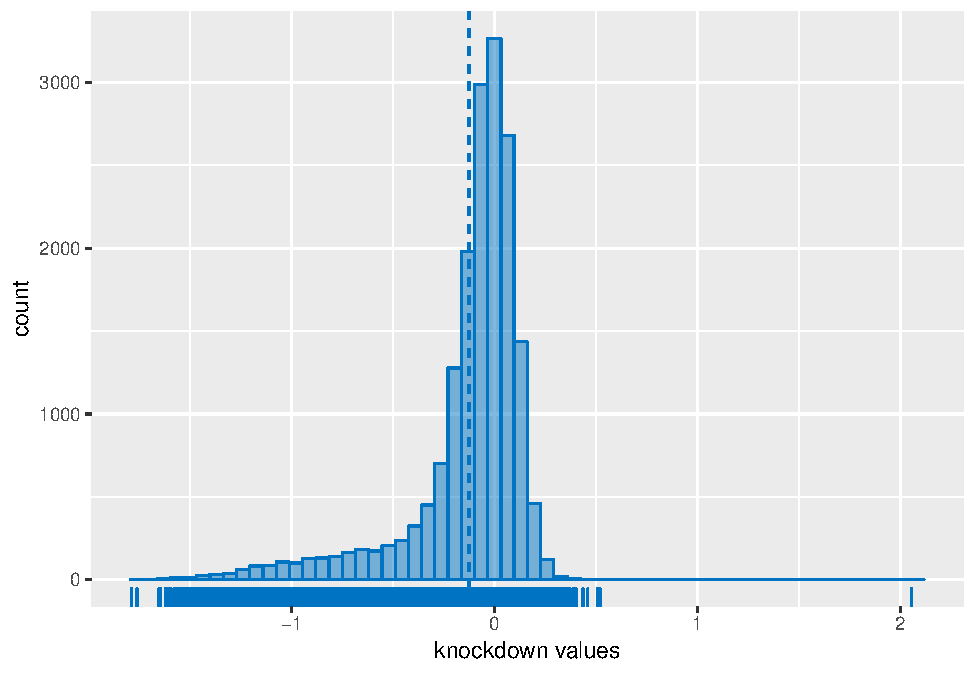
\includegraphics{Project_HNC_files/figure-latex/1_knockdown_values2-1.pdf}

To check if there are more essential genes in HNC, the means of HNC
patients with the reference group were compared.

\begin{Shaded}
\begin{Highlighting}[]
\CommentTok{# Are there genes that tend to be more essential in HNC?}
\NormalTok{esgene1 =}\StringTok{ }\NormalTok{kd.ceres.HNC[}\KeywordTok{which}\NormalTok{(}\KeywordTok{rowMeans}\NormalTok{(kd.ceres.HNC)}\OperatorTok{<}\StringTok{ }\KeywordTok{rowMeans}\NormalTok{(kd.ceres.reference)),]}
\CommentTok{# Sort essential genes}
\NormalTok{esgene1=}\StringTok{ }\NormalTok{esgene1[}\KeywordTok{order}\NormalTok{(}\KeywordTok{rowMeans}\NormalTok{(esgene1)),]}
\end{Highlighting}
\end{Shaded}

\subsubsection{Example EGFR}\label{example-egfr}

Checking the summary of an example gene

\begin{Shaded}
\begin{Highlighting}[]
\CommentTok{# Transposition of dataframe esgene1}
\NormalTok{esgeneT =}\StringTok{ }\KeywordTok{as.data.frame}\NormalTok{(}\KeywordTok{t}\NormalTok{(esgene1))}
\KeywordTok{summary}\NormalTok{(esgeneT}\OperatorTok{$}\NormalTok{EGFR)}
\end{Highlighting}
\end{Shaded}

\begin{verbatim}
   Min. 1st Qu.  Median    Mean 3rd Qu.    Max. 
-0.9636 -0.5200 -0.4221 -0.4097 -0.2866  0.0189 
\end{verbatim}

\subsubsection{Boxplot of 20 random
genes}\label{boxplot-of-20-random-genes}

\begin{Shaded}
\begin{Highlighting}[]
\CommentTok{# Boxplot of 20 of most significiant genes according to knockdown analysis}
\KeywordTok{boxplot}\NormalTok{(}\KeywordTok{sample}\NormalTok{(esgeneT,}\DecValTok{20}\NormalTok{, }\DataTypeTok{replace =} \OtherTok{FALSE}\NormalTok{), }\DataTypeTok{xlab =} \StringTok{"gene"}\NormalTok{, }\DataTypeTok{horizontal =}\NormalTok{T, }\DataTypeTok{main=}\StringTok{"Knockdown values of 20 random genes"}\NormalTok{,}
        \DataTypeTok{xlab=}\StringTok{"genes"}\NormalTok{,}
        \DataTypeTok{ylab=}\StringTok{"Knockdown values"}\NormalTok{,}
        \DataTypeTok{col=}\StringTok{"blue"}\NormalTok{,}
        \DataTypeTok{border=}\StringTok{"brown"}\NormalTok{,}
        \DataTypeTok{outline =} \OtherTok{TRUE}\NormalTok{,}
        \DataTypeTok{notch =} \OtherTok{TRUE}\NormalTok{)}
\KeywordTok{abline}\NormalTok{(}\DataTypeTok{col =} \KeywordTok{c}\NormalTok{(}\StringTok{"blue"}\NormalTok{, }\StringTok{"red"}\NormalTok{, }\StringTok{"black"}\NormalTok{, }\StringTok{"orange"}\NormalTok{),}
        \DataTypeTok{lty =} \DecValTok{2}\NormalTok{)}
\end{Highlighting}
\end{Shaded}

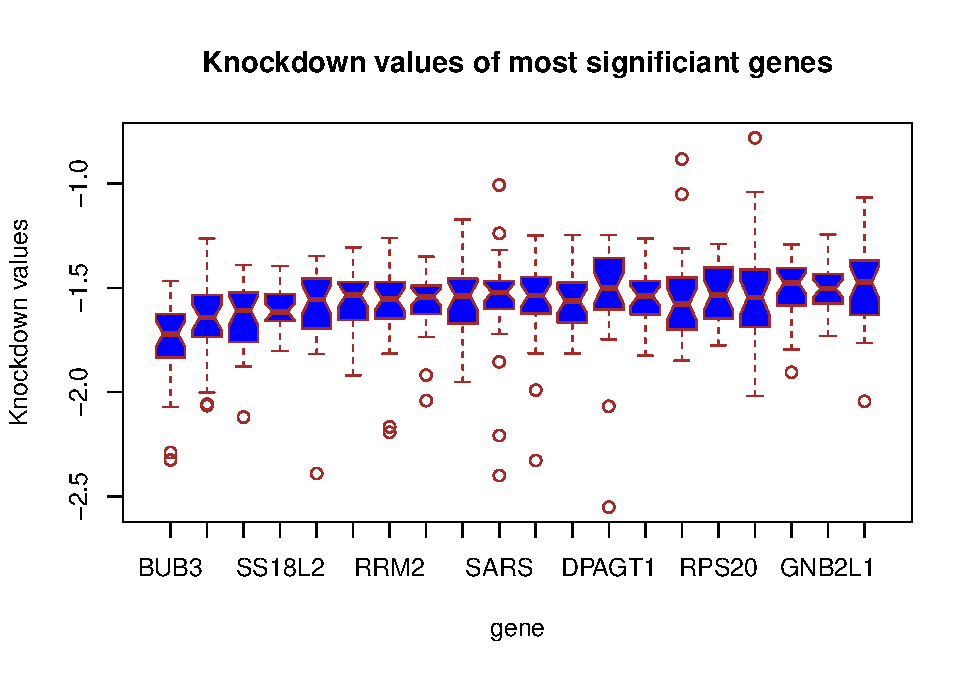
\includegraphics{Project_HNC_files/figure-latex/1_knockdown_boxplot-1.pdf}

\subsubsection{Applying Wilcoxon rank sum test because knockdown values
are not normally
distributed}\label{applying-wilcoxon-rank-sum-test-because-knockdown-values-are-not-normally-distributed}

To check if the HNC knockdown values differ from the compare group, a
wilcoxon test is executed.

\begin{Shaded}
\begin{Highlighting}[]
\KeywordTok{wilcox.test}\NormalTok{(mean.kd.ceres.HNC, mean.kd.ceres.reference)}
\end{Highlighting}
\end{Shaded}

\begin{verbatim}

    Wilcoxon rank sum test with continuity correction

data:  mean.kd.ceres.HNC and mean.kd.ceres.reference
W = 155160000, p-value = 0.7421
alternative hypothesis: true location shift is not equal to 0
\end{verbatim}

The test shows, that ther isn`t a significiant difference between HNC
patients and the reference group. Due to the fact, that knocking down of
essential genes has the same effect in healthy cells, than in tumorous
cells.

\subsubsection{Cleanup of the
enviroment}\label{cleanup-of-the-enviroment-2}

\begin{Shaded}
\begin{Highlighting}[]
\KeywordTok{rm}\NormalTok{(kd.ceres.HNC.dist, kd.ceres.reference, kd.ceres.reference.dist, mean.kd.ceres.HNC, mean.kd.ceres.reference, mean.kd.ceres.dist, esgene1, esgeneT)}
\end{Highlighting}
\end{Shaded}

\section{2. Identify genes of
interest}\label{identify-genes-of-interest}

\subsection{k-means clustering of CNA and expression data with
normalized values(-reference) for SDL
GOI}\label{k-means-clustering-of-cna-and-expression-data-with-normalized-values-reference-for-sdl-goi}

To find potential genes for SDL pair detection, clustering through
k-means was executed.

\begin{Shaded}
\begin{Highlighting}[]
\NormalTok{km.genes =}\StringTok{ }\KeywordTok{Reduce}\NormalTok{(intersect, }\KeywordTok{list}\NormalTok{(}\KeywordTok{rownames}\NormalTok{(expression.HNC), }\KeywordTok{rownames}\NormalTok{(copynumber.HNC))) }\CommentTok{# Intersect set of expression and CNA}

\CommentTok{# Create data rame with expression and CNA values}
\NormalTok{km.expression =}\StringTok{ }\NormalTok{expr.HNC.norm[km.genes,]}
\NormalTok{km.copynumber =}\StringTok{ }\NormalTok{cna.HNC.norm[km.genes,]}
\NormalTok{km.data =}\StringTok{ }\KeywordTok{lapply}\NormalTok{(}\DecValTok{1}\OperatorTok{:}\KeywordTok{length}\NormalTok{(ID), }\ControlFlowTok{function}\NormalTok{(x) \{}
\NormalTok{  out =}\StringTok{ }\KeywordTok{data.frame}\NormalTok{(}\DataTypeTok{genes =}\NormalTok{km.genes, }\DataTypeTok{expression =}\NormalTok{ km.expression[,x], }\DataTypeTok{copynumber =}\NormalTok{ km.copynumber[,x])}
  \KeywordTok{return}\NormalTok{ (out)}
\NormalTok{\})}
\CommentTok{# Combine rows for k mean clustering}
\NormalTok{comb.ex.cna =}\StringTok{ }\KeywordTok{do.call}\NormalTok{(rbind, km.data)}
\NormalTok{comb.ex.cna =}\StringTok{ }\NormalTok{comb.ex.cna[}\KeywordTok{which}\NormalTok{(comb.ex.cna}\OperatorTok{$}\NormalTok{copynumber }\OperatorTok{>=}\StringTok{ }\DecValTok{1} \OperatorTok{&}\StringTok{ }\NormalTok{comb.ex.cna}\OperatorTok{$}\NormalTok{expression }\OperatorTok{>=}\KeywordTok{quantile}\NormalTok{(comb.ex.cna}\OperatorTok{$}\NormalTok{expression,}\FloatTok{0.95}\NormalTok{)),]}

\CommentTok{# Plotting of normalized expression valuess against CNA data for a short overview. }
\KeywordTok{ggplot}\NormalTok{(comb.ex.cna[, }\DecValTok{2}\OperatorTok{:}\DecValTok{3}\NormalTok{],}
       \KeywordTok{aes}\NormalTok{(}\DataTypeTok{x =}\NormalTok{ expression, }\DataTypeTok{y =}\NormalTok{ copynumber, }\DataTypeTok{color =} \StringTok{"smooth"}\NormalTok{)) }\OperatorTok{+}
\StringTok{  }\KeywordTok{geom_point}\NormalTok{()}
\end{Highlighting}
\end{Shaded}

\includegraphics{Project_HNC_files/figure-latex/2_kmeans-1.pdf}

To check the perfect ammount of clusters in k-means, an ellbow test was
implemented.

\begin{Shaded}
\begin{Highlighting}[]
\CommentTok{# Ellbow method to find optimal ammount of clusters}
\NormalTok{emp =}\StringTok{ }\KeywordTok{vector}\NormalTok{() }\CommentTok{# Create an empty vector}
\ControlFlowTok{for}\NormalTok{ (i }\ControlFlowTok{in} \DecValTok{1}\OperatorTok{:}\DecValTok{10}\NormalTok{) emp[i] =}\StringTok{ }\KeywordTok{sum}\NormalTok{(}\KeywordTok{kmeans}\NormalTok{(comb.ex.cna[}\DecValTok{2}\OperatorTok{:}\DecValTok{3}\NormalTok{], i)}\OperatorTok{$}\NormalTok{withinss) }\CommentTok{# Calculate the sum within squared values for 10 clusters}
\NormalTok{emp }\CommentTok{# Look at the sum within squares for 10 clusters}
\end{Highlighting}
\end{Shaded}

\begin{verbatim}
 [1] 2607.5505 1461.2845  927.0961  706.2404  590.1994  415.6683  350.4004
 [8]  311.1543  273.6164  252.6120
\end{verbatim}

\begin{Shaded}
\begin{Highlighting}[]
\CommentTok{# Plotting of Ellbow method}
\KeywordTok{plot}\NormalTok{(}\DecValTok{1}\OperatorTok{:}\DecValTok{10}\NormalTok{,}
\NormalTok{     emp,}
     \DataTypeTok{type =} \StringTok{'b'}\NormalTok{,}
     \DataTypeTok{main =} \KeywordTok{paste}\NormalTok{(}\StringTok{'The Elbow Method'}\NormalTok{),}
     \DataTypeTok{xlab =} \StringTok{'Number of clusters'}\NormalTok{,}
     \DataTypeTok{ylab =} \StringTok{'EMP'}\NormalTok{) }
\end{Highlighting}
\end{Shaded}

\includegraphics{Project_HNC_files/figure-latex/2_ellbow method-1.pdf}

Result: The ellbow test shows that 3 clusters are sufficient.

K-means were executed and plotted. Afterwards the potential SDL
candidates were identified through higher expression values.

\begin{Shaded}
\begin{Highlighting}[]
\CommentTok{# Fitting K-Means to the dataset}
\NormalTok{kmeans =}\StringTok{ }\KeywordTok{kmeans}\NormalTok{(}\DataTypeTok{x =}\NormalTok{ comb.ex.cna[,}\DecValTok{2}\OperatorTok{:}\DecValTok{3}\NormalTok{], }\DataTypeTok{centers =} \DecValTok{3}\NormalTok{,}\DataTypeTok{iter.max =} \DecValTok{1000}\NormalTok{, }\DataTypeTok{nstart =} \DecValTok{1}\NormalTok{) }\CommentTok{# See elbow method (k = 3) }
\NormalTok{y_kmeans =}\StringTok{ }\NormalTok{kmeans}\OperatorTok{$}\NormalTok{cluster }

\CommentTok{# Visualising the clusters}
\KeywordTok{clusplot}\NormalTok{(comb.ex.cna,}
\NormalTok{         y_kmeans,}
         \DataTypeTok{lines =} \DecValTok{0}\NormalTok{,}
         \DataTypeTok{shade =} \OtherTok{TRUE}\NormalTok{,}
         \DataTypeTok{color =} \OtherTok{TRUE}\NormalTok{,}
         \DataTypeTok{labels =} \DecValTok{4}\NormalTok{,}
         \DataTypeTok{plotchar =} \OtherTok{FALSE}\NormalTok{,}
         \DataTypeTok{span =} \OtherTok{TRUE}\NormalTok{,}
         \DataTypeTok{stand =} \OtherTok{FALSE}\NormalTok{,}
         \DataTypeTok{cex =}\FloatTok{0.5}\NormalTok{,}
         \DataTypeTok{main =} \KeywordTok{paste}\NormalTok{(}\StringTok{'Clusters of Genes'}\NormalTok{),}
         \DataTypeTok{xlab =} \StringTok{'Expression'}\NormalTok{,}
         \DataTypeTok{ylab =} \StringTok{'CNA'}\NormalTok{)}
\end{Highlighting}
\end{Shaded}

\includegraphics{Project_HNC_files/figure-latex/2_kmeansclustering-1.pdf}

The Plot ``Cluster of genes'' features the 3 clusters of values from
expression and CNA data. Due to little variance between the data pairs,
the intersection set is comparatively big.

In order to define SDL candidates, the cluster with highest expression
values was chosen and filtered again according to expression numbers.

\begin{Shaded}
\begin{Highlighting}[]
\NormalTok{comb.ex.cna =}\StringTok{ }\KeywordTok{cbind}\NormalTok{(comb.ex.cna, y_kmeans)}\CommentTok{# Combine kmeans with genes}
\CommentTok{# Sort comb.ex.cna data decresing for selecting adequate number of cluster}
\NormalTok{comb.ex.cna =}\StringTok{ }\NormalTok{comb.ex.cna[}\KeywordTok{order}\NormalTok{(comb.ex.cna}\OperatorTok{$}\NormalTok{expression,}\DataTypeTok{decreasing =}\OtherTok{TRUE}\NormalTok{),]}

\CommentTok{# Filtering of the most expressed and alterated genes}
\NormalTok{goi.sdl =}\StringTok{ }\NormalTok{comb.ex.cna[}\KeywordTok{which}\NormalTok{(comb.ex.cna}\OperatorTok{$}\NormalTok{y_kmeans }\OperatorTok{==}\StringTok{ }\NormalTok{comb.ex.cna[}\DecValTok{1}\NormalTok{,}\DecValTok{4}\NormalTok{]),]}

\CommentTok{# Sort dataframe }
\NormalTok{goi.sdl =}\StringTok{ }\NormalTok{goi.sdl[}\KeywordTok{order}\NormalTok{(goi.sdl}\OperatorTok{$}\NormalTok{expression,}\DataTypeTok{decreasing=}\OtherTok{TRUE}\NormalTok{),]}
\KeywordTok{kable}\NormalTok{(goi.sdl[}\DecValTok{1}\OperatorTok{:}\DecValTok{5}\NormalTok{,])}
\end{Highlighting}
\end{Shaded}

\begin{longtable}[]{@{}llrrr@{}}
\toprule
& genes & expression & copynumber & y\_kmeans\tabularnewline
\midrule
\endhead
428012 & DSG3 & 8.237872 & 1.641760 & 2\tabularnewline
41915 & FXYD3 & 7.914724 & 1.022479 & 2\tabularnewline
33343 & CST6 & 7.484452 & 1.372464 & 2\tabularnewline
185157 & F3 & 7.466245 & 1.610442 & 2\tabularnewline
354894 & FOXE1 & 7.447917 & 3.676721 & 2\tabularnewline
\bottomrule
\end{longtable}

\begin{Shaded}
\begin{Highlighting}[]
\NormalTok{goi.SDL =}\StringTok{ }\KeywordTok{as.character}\NormalTok{(goi.sdl}\OperatorTok{$}\NormalTok{genes[}\DecValTok{1}\OperatorTok{:}\DecValTok{5}\NormalTok{])}
\KeywordTok{rm}\NormalTok{(emp, i, km.genes, y_kmeans, kmeans, km.copynumber, km.data, km.expression, comb.ex.cna) }\CommentTok{# Clean enviroment}
\end{Highlighting}
\end{Shaded}

\subsection{Investigate high frequencies of deleterious mutations SL
GOI}\label{investigate-high-frequencies-of-deleterious-mutations-sl-goi}

Create a dataframe with data for the heatmap.

\begin{Shaded}
\begin{Highlighting}[]
\NormalTok{mutation.HNC.df =}\StringTok{ }\KeywordTok{do.call}\NormalTok{(rbind, mutation.HNC) }\CommentTok{# All mutation data of HNC samples in one dataframe}
\NormalTok{heatmap.genes =}\StringTok{ }\KeywordTok{as.data.frame}\NormalTok{(}\KeywordTok{table}\NormalTok{(mutation.HNC.df}\OperatorTok{$}\NormalTok{Hugo_Symbol)) }\CommentTok{# Dataframe with all mutated genes in HNC samples just once}

\NormalTok{heatmap.data =}\StringTok{ }\KeywordTok{as.data.frame}\NormalTok{(}\KeywordTok{sapply}\NormalTok{(}\DecValTok{1}\OperatorTok{:}\NormalTok{(}\KeywordTok{length}\NormalTok{(ID)), }\ControlFlowTok{function}\NormalTok{(a) \{}
\NormalTok{  out =}\StringTok{ }\KeywordTok{ifelse}\NormalTok{(heatmap.genes}\OperatorTok{$}\NormalTok{Var1 }\OperatorTok\StringTok{ }\NormalTok{mutation.HNC[[a]]}\OperatorTok{$}\NormalTok{Hugo_Symbol, }\DecValTok{1}\NormalTok{, }\DecValTok{0}\NormalTok{) }\CommentTok{# Per HNC sample: every gene which is mutated gets a 1, otherwise a 0}
  \KeywordTok{return}\NormalTok{(out)}
\NormalTok{\}))}

\CommentTok{# Define row and column names}
\KeywordTok{rownames}\NormalTok{(heatmap.data) =}\StringTok{ }\NormalTok{heatmap.genes}\OperatorTok{$}\NormalTok{Var1}
\KeywordTok{colnames}\NormalTok{(heatmap.data) =}\StringTok{ }\NormalTok{ID}

\CommentTok{# Order from high to low frequency}
\NormalTok{heatmap.data}\OperatorTok{$}\NormalTok{sum =}\StringTok{ }\KeywordTok{apply}\NormalTok{(heatmap.data, }\DecValTok{1}\NormalTok{, sum)}
\NormalTok{heatmap.data =}\StringTok{ }\NormalTok{heatmap.data[}\KeywordTok{order}\NormalTok{(}\OperatorTok{-}\NormalTok{heatmap.data}\OperatorTok{$}\NormalTok{sum), }\DecValTok{1}\OperatorTok{:}\DecValTok{27}\NormalTok{] }

\CommentTok{# Heatmap of the most frequently deleterious mutated genes in HNC samples}
\KeywordTok{heatmap}\NormalTok{(}\KeywordTok{data.matrix}\NormalTok{(heatmap.data)[}\DecValTok{1}\OperatorTok{:}\DecValTok{40}\NormalTok{,],}
        \DataTypeTok{Rowv=}\OtherTok{NA}\NormalTok{,}
        \DataTypeTok{Colv=}\OtherTok{NA}\NormalTok{,}
        \DataTypeTok{col =} \KeywordTok{c}\NormalTok{(}\StringTok{"lightgrey"}\NormalTok{, }\StringTok{"tomato2"}\NormalTok{),}
        \DataTypeTok{scale=}\StringTok{"column"}\NormalTok{,}
        \DataTypeTok{cexRow =} \FloatTok{0.8}\NormalTok{,}
        \DataTypeTok{cexCol =} \FloatTok{0.8}\NormalTok{,}
        \DataTypeTok{main =} \StringTok{"Most frequently deleterious mutated genes in HNC samples"}\NormalTok{)}
\end{Highlighting}
\end{Shaded}

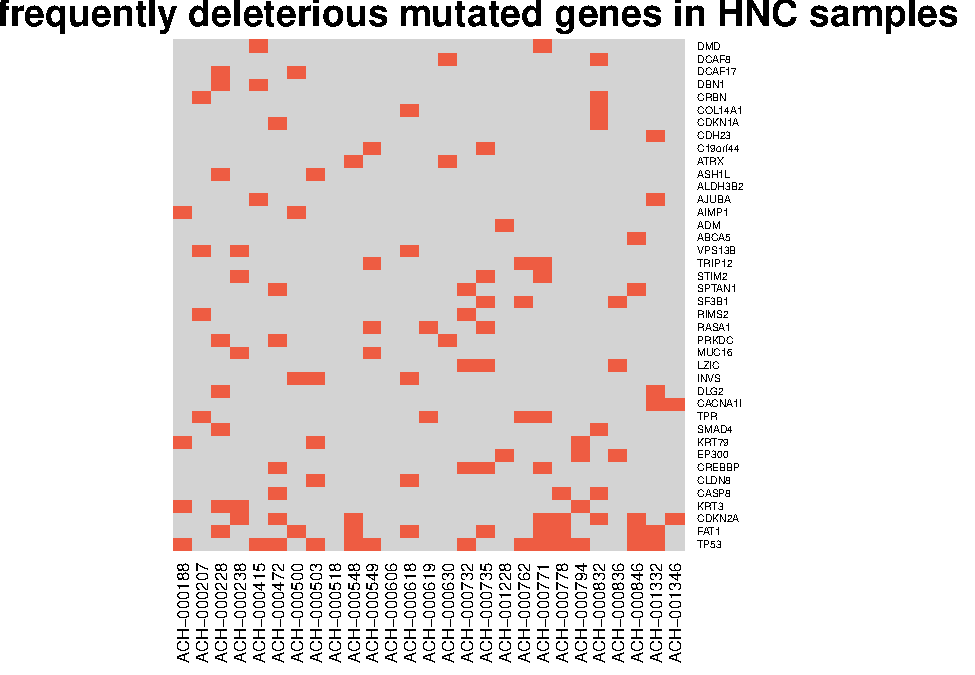
\includegraphics{Project_HNC_files/figure-latex/2_SLgoi1-1.pdf}

Result: TP53, FAT1, CDKN2A, KRT3 and CASP8 are the 5 most frequently
deleterious mutated genes in our HNC samples

According to Leemans et al. (2018) these are frequent mutations in HNC:
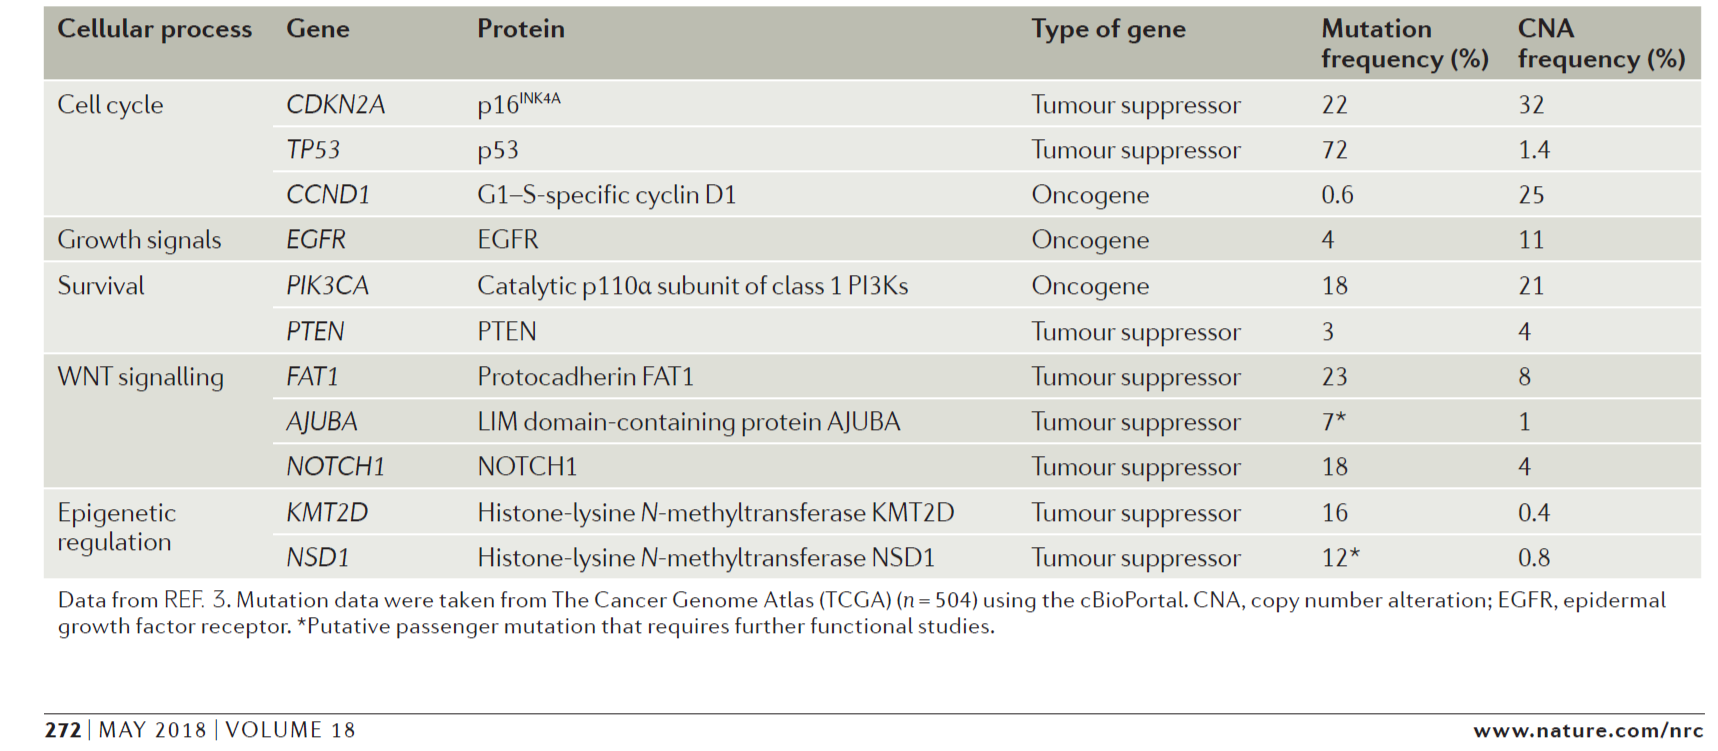
\includegraphics{images/frequent_mutations_HNC.png}

Leemans, C. R. et al. (2018). The molecular landscape of head and neck
cancer. Nat. Rev.~Cancer 18, 269-282.

Compare our SL GOI with genes from literature.

\begin{Shaded}
\begin{Highlighting}[]
\CommentTok{# create dataframe with goi from literature}
\NormalTok{goi.lit =}\StringTok{ }\KeywordTok{data.frame}\NormalTok{(}\DataTypeTok{Gene =} \KeywordTok{c}\NormalTok{(}\StringTok{"CDKN2A"}\NormalTok{, }\StringTok{"TP53"}\NormalTok{, }\StringTok{"CCND1"}\NormalTok{, }\StringTok{"EGFR"}\NormalTok{, }\StringTok{"PIK3CA"}\NormalTok{, }\StringTok{"PTEN"}\NormalTok{, }\StringTok{"FAT1"}\NormalTok{, }\StringTok{"AJUBA"}\NormalTok{, }\StringTok{"NOTCH1"}\NormalTok{, }\StringTok{"KMT2D"}\NormalTok{, }\StringTok{"NSD1"}\NormalTok{),}
                     \StringTok{"Mutation frequency"}\NormalTok{ =}\StringTok{ }\KeywordTok{c}\NormalTok{(}\DecValTok{22}\NormalTok{, }\DecValTok{72}\NormalTok{, }\FloatTok{0.6}\NormalTok{, }\DecValTok{4}\NormalTok{, }\DecValTok{18}\NormalTok{, }\DecValTok{3}\NormalTok{, }\DecValTok{23}\NormalTok{, }\DecValTok{7}\NormalTok{, }\DecValTok{18}\NormalTok{, }\DecValTok{16}\NormalTok{, }\DecValTok{12}\NormalTok{),}
                     \StringTok{"CNA frequency"}\NormalTok{ =}\StringTok{ }\KeywordTok{c}\NormalTok{(}\DecValTok{32}\NormalTok{, }\FloatTok{1.4}\NormalTok{, }\DecValTok{25}\NormalTok{, }\DecValTok{11}\NormalTok{, }\DecValTok{21}\NormalTok{, }\DecValTok{4}\NormalTok{, }\DecValTok{8}\NormalTok{, }\DecValTok{1}\NormalTok{, }\DecValTok{4}\NormalTok{, }\FloatTok{0.4}\NormalTok{, }\FloatTok{0.8}\NormalTok{)) }

\NormalTok{heatmap_position =}\StringTok{ }\KeywordTok{sapply}\NormalTok{(}\DecValTok{1}\OperatorTok{:}\KeywordTok{nrow}\NormalTok{(goi.lit), }\ControlFlowTok{function}\NormalTok{(a) \{ }\CommentTok{# Search for the position of goi.lit in mutated genes of HNC samples}
\NormalTok{  position =}\StringTok{ }\KeywordTok{which}\NormalTok{(}\KeywordTok{rownames}\NormalTok{(heatmap.data) }\OperatorTok{==}\StringTok{ }\NormalTok{goi.lit}\OperatorTok{$}\NormalTok{Gene[a])}
  \ControlFlowTok{if}\NormalTok{(}\KeywordTok{length}\NormalTok{(position) }\OperatorTok{==}\StringTok{ }\DecValTok{0}\NormalTok{) \{position =}\StringTok{ }\OtherTok{NA}\NormalTok{\} }\CommentTok{# If gene is not part of the genes mutated in HNC samples its position is replaced with NA}
  \KeywordTok{return}\NormalTok{(position)}
\NormalTok{\})}

\NormalTok{goi.lit}\OperatorTok{$}\StringTok{"Heatmap position"}\NormalTok{ =}\StringTok{ }\NormalTok{heatmap_position }\CommentTok{# Add heatmap position to goi.lit}
\KeywordTok{rownames}\NormalTok{(goi.lit) =}\StringTok{ }\NormalTok{goi.lit}\OperatorTok{$}\NormalTok{Gene}
\NormalTok{goi.lit}\OperatorTok{$}\NormalTok{Gene =}\StringTok{ }\OtherTok{NULL}
\NormalTok{goi.lit =}\StringTok{ }\NormalTok{goi.lit[}\KeywordTok{order}\NormalTok{(goi.lit}\OperatorTok{$}\StringTok{"Heatmap position"}\NormalTok{),]}
\KeywordTok{kable}\NormalTok{(goi.lit) }\CommentTok{# Show a table of goi.lit}
\end{Highlighting}
\end{Shaded}

\begin{longtable}[]{@{}lrrr@{}}
\toprule
& Mutation.frequency & CNA.frequency & Heatmap position\tabularnewline
\midrule
\endhead
TP53 & 72.0 & 1.4 & 1\tabularnewline
FAT1 & 23.0 & 8.0 & 2\tabularnewline
CDKN2A & 22.0 & 32.0 & 3\tabularnewline
AJUBA & 7.0 & 1.0 & 28\tabularnewline
KMT2D & 16.0 & 0.4 & 66\tabularnewline
NOTCH1 & 18.0 & 4.0 & 82\tabularnewline
NSD1 & 12.0 & 0.8 & 715\tabularnewline
CCND1 & 0.6 & 25.0 & NA\tabularnewline
EGFR & 4.0 & 11.0 & NA\tabularnewline
PIK3CA & 18.0 & 21.0 & NA\tabularnewline
PTEN & 3.0 & 4.0 & NA\tabularnewline
\bottomrule
\end{longtable}

Because our most frequent mutated genes almost aproximately match with
frequent mutations from literature we choose the 5 genes with most
frequent mutations in HNC samples.

\begin{Shaded}
\begin{Highlighting}[]
\NormalTok{goi.SL =}\StringTok{ }\KeywordTok{rownames}\NormalTok{(heatmap.data)[}\DecValTok{1}\OperatorTok{:}\DecValTok{5}\NormalTok{]}
\NormalTok{goi.SL}
\end{Highlighting}
\end{Shaded}

\begin{verbatim}
[1] "TP53"   "FAT1"   "CDKN2A" "KRT3"   "CASP8" 
\end{verbatim}

Clean up of the enviroment

\begin{Shaded}
\begin{Highlighting}[]
\KeywordTok{rm}\NormalTok{(mutation.HNC.df, heatmap.genes, heatmap.data, heatmap_position)}
\end{Highlighting}
\end{Shaded}

\section{3. Find SL/SDL partner}\label{find-slsdl-partner}

\subsection{SL/SDL partner search following the daisy
model}\label{slsdl-partner-search-following-the-daisy-model}

To examine gene pairs A and B which fulfill the criteria of SoF and
functional examination we performe a Wilcoxon rank sum test on
copynumber or CERES knockdown data. We have 5 inactive genes (goi.SL)
and 5 overactive genes (goi.SDL) which are defined as genes A. The
Wilcoxon rank sum test now returns all genes B which pass the test in a
significant manner (p\textless{}0.05).

\begin{Shaded}
\begin{Highlighting}[]
\StringTok{'Daisy.Wilcox'}\NormalTok{ =}\StringTok{ }\ControlFlowTok{function}\NormalTok{(input_genes,input_data, inactive_overactive, less_greater)\{}
\NormalTok{  Daisy_Wilcox =}\StringTok{ }\KeywordTok{lapply}\NormalTok{(}\DecValTok{1}\OperatorTok{:}\KeywordTok{length}\NormalTok{(input_genes), }\ControlFlowTok{function}\NormalTok{(m) \{}
\NormalTok{  goi =}\StringTok{ }\NormalTok{input_genes[m] }\CommentTok{# Set 1 of 5 goi}
  \CommentTok{# Depending on SL or SDL partner search gene B needs to be inactive (SL) or overactive (SDL)}
  \ControlFlowTok{if}\NormalTok{(inactive_overactive }\OperatorTok{==}\StringTok{ }\DecValTok{1}\NormalTok{) \{ }\CommentTok{# inactive_overactive == 1 chooses overactive}
\NormalTok{    mean.exp.goi =}\StringTok{ }\KeywordTok{mean}\NormalTok{(}\KeywordTok{t}\NormalTok{(expression[goi,]))}
\NormalTok{    exp.goi.norm =}\StringTok{ }\NormalTok{expression[goi,] }\OperatorTok{-}\StringTok{ }\NormalTok{mean.exp.goi }\CommentTok{# Normalised expression values of goi}
\NormalTok{    mut_overa.ID =}\StringTok{ }\KeywordTok{lapply}\NormalTok{(}\DecValTok{1}\OperatorTok{:}\KeywordTok{ncol}\NormalTok{(expression), }\ControlFlowTok{function}\NormalTok{(a) \{}
\NormalTok{    out =}\StringTok{ }\ControlFlowTok{if}\NormalTok{(exp.goi.norm[goi, a] }\OperatorTok{>}\StringTok{ }\DecValTok{0} \OperatorTok{&}\StringTok{ }\NormalTok{copynumber[goi,a] }\OperatorTok{>}\StringTok{ }\FloatTok{0.3}\NormalTok{) \{a\} }\ControlFlowTok{else}\NormalTok{ \{}\OtherTok{NA}\NormalTok{\} }\CommentTok{# Filter all IDs which are overactive: overexpressed and CNA > 0,3}
    \KeywordTok{return}\NormalTok{(out)}
\NormalTok{    \})}
\NormalTok{  \} }\ControlFlowTok{else}\NormalTok{ \{ }\CommentTok{# inactive_overactive == 0 chooses inactive}
\NormalTok{    mut_overa.ID =}\StringTok{ }\KeywordTok{lapply}\NormalTok{(}\DecValTok{1}\OperatorTok{:}\KeywordTok{length}\NormalTok{(mutation), }\ControlFlowTok{function}\NormalTok{(a) \{}
\NormalTok{    out =}\StringTok{ }\KeywordTok{ifelse}\NormalTok{(goi }\OperatorTok\StringTok{ }\NormalTok{mutation[[a]]}\OperatorTok{$}\NormalTok{Hugo_Symbol, a, }\OtherTok{NA}\NormalTok{) }\CommentTok{# Filter all IDs which have a mutation of goi}
    \KeywordTok{return}\NormalTok{(out)}
\NormalTok{    \})}
\NormalTok{  \}}
  
\NormalTok{  not_mut_overa.ID =}\StringTok{ }\KeywordTok{grep}\NormalTok{(}\StringTok{"NA"}\NormalTok{, mut_overa.ID) }\CommentTok{# ID of samples which have NO inactivity/overactivity of goi}
\NormalTok{  mut_overa.ID =}\StringTok{ }\KeywordTok{as.integer}\NormalTok{(mut_overa.ID[}\KeywordTok{is.na}\NormalTok{(mut_overa.ID) }\OperatorTok{==}\StringTok{ }\OtherTok{FALSE}\NormalTok{]) }\CommentTok{# ID of samples which HAVE inactivity/overactivity of goi}

\NormalTok{  p.value =}\StringTok{ }\KeywordTok{sapply}\NormalTok{(}\DecValTok{1}\OperatorTok{:}\KeywordTok{nrow}\NormalTok{(input_data), }\ControlFlowTok{function}\NormalTok{(b) \{}
\NormalTok{    mut_overa.data =}\StringTok{ }\KeywordTok{t}\NormalTok{(input_data[b, mut_overa.ID])}
\NormalTok{    not_mut_overa.data =}\StringTok{ }\KeywordTok{t}\NormalTok{(input_data[b, not_mut_overa.ID])}
    \ControlFlowTok{if}\NormalTok{ (less_greater }\OperatorTok{==}\StringTok{ }\DecValTok{1}\NormalTok{) \{}
\NormalTok{      p =}\StringTok{ }\KeywordTok{wilcox.test}\NormalTok{(mut_overa.data, not_mut_overa.data, }\DataTypeTok{alternative =} \StringTok{"greater"}\NormalTok{)}\OperatorTok{$}\NormalTok{p.value }\CommentTok{# One sided (greater) Wilcoxon Sum Rank Test }
\NormalTok{    \} }\ControlFlowTok{else}\NormalTok{ \{}
\NormalTok{      p =}\StringTok{ }\KeywordTok{wilcox.test}\NormalTok{(mut_overa.data, not_mut_overa.data, }\DataTypeTok{alternative =} \StringTok{"less"}\NormalTok{)}\OperatorTok{$}\NormalTok{p.value }\CommentTok{# One sided (greater) Wilcoxon Sum Rank Test}
\NormalTok{    \}}
    
\NormalTok{  \})}

\NormalTok{  out =}\StringTok{ }\KeywordTok{data.frame}\NormalTok{(}\DataTypeTok{genes =} \KeywordTok{rownames}\NormalTok{(input_data), }\DataTypeTok{p_value =}\NormalTok{ p.value)}
\NormalTok{  out =}\StringTok{ }\NormalTok{out[}\KeywordTok{which}\NormalTok{(out}\OperatorTok{$}\NormalTok{p_value }\OperatorTok{<}\StringTok{ }\FloatTok{0.05}\NormalTok{),]}
  \KeywordTok{return}\NormalTok{(out)}
\NormalTok{  \})}
  \KeywordTok{names}\NormalTok{(Daisy_Wilcox) =}\StringTok{ }\NormalTok{input_genes}
  \KeywordTok{return}\NormalTok{(Daisy_Wilcox)}
\NormalTok{\}}
\end{Highlighting}
\end{Shaded}

To examine gene pairs A and B which fulfill the criteria of gene co
expresssion we performe a Spearman correlation test on the expression
data. We have 5 inactive genes (goi.SL) and 5 overactive genes (goi.SDL)
which are defined as genes A The correlation test now returns all genes
B that correlate to gene A in a significant manner (p\textless{}0.05).

\begin{Shaded}
\begin{Highlighting}[]
\StringTok{'Daisy.Spearman'}\NormalTok{ =}\StringTok{ }\ControlFlowTok{function}\NormalTok{(input_genes)\{}
\NormalTok{  Daisy_Spearman =}\StringTok{ }\KeywordTok{lapply}\NormalTok{(}\DecValTok{1}\OperatorTok{:}\KeywordTok{length}\NormalTok{(input_genes), }\ControlFlowTok{function}\NormalTok{(m) \{ }\CommentTok{# Build up a list with the 5 goi; lapply: goes through the code for each gene A}
\NormalTok{  goi =}\StringTok{ }\NormalTok{input_genes[m]}

\NormalTok{  p.value =}\StringTok{ }\KeywordTok{sapply}\NormalTok{(}\DecValTok{1}\OperatorTok{:}\KeywordTok{nrow}\NormalTok{(expression), }\ControlFlowTok{function}\NormalTok{(a)\{  }\CommentTok{# Creation of a list with the length of the expression data, for the reacent goi, go through every gene and calculate cor.test}
\NormalTok{    expression.goi =}\KeywordTok{t}\NormalTok{(expression[goi,])           }\CommentTok{# Variable containing expressiondata of the goi (gene A)}
\NormalTok{    expression.GeneB =}\KeywordTok{t}\NormalTok{(expression[a,])           }\CommentTok{# Variable containing all other genes (gene B)}
\NormalTok{    p =}\StringTok{ }\KeywordTok{cor.test}\NormalTok{(expression.goi,expression.GeneB, }\DataTypeTok{alternative =} \StringTok{"greater"}\NormalTok{, }\DataTypeTok{method =} \StringTok{"spearman"}\NormalTok{, }\DataTypeTok{exact =} \OtherTok{FALSE}\NormalTok{)}\OperatorTok{$}\NormalTok{p.value }\CommentTok{# One sided spearman correlation test  }
\NormalTok{  \})}
  
  \CommentTok{# Return a dataframe with the columns genes(HugoSymbols) and p_values (p.values)}
\NormalTok{  out =}\StringTok{ }\KeywordTok{data.frame}\NormalTok{(}\DataTypeTok{genes =} \KeywordTok{rownames}\NormalTok{(expression), }\DataTypeTok{p_value =}\NormalTok{ p.value)}
\NormalTok{  out =}\StringTok{ }\NormalTok{out[}\KeywordTok{which}\NormalTok{(out}\OperatorTok{$}\NormalTok{p_value }\OperatorTok{<}\StringTok{ }\FloatTok{0.05}\NormalTok{),] }\CommentTok{# Filter for significant p.values}
\NormalTok{  out =}\StringTok{ }\NormalTok{out[}\KeywordTok{which}\NormalTok{(out}\OperatorTok{$}\NormalTok{genes }\OperatorTok{!=}\StringTok{ }\NormalTok{goi),]   }\CommentTok{# Select onl these wich are not the same gene as the goi (would be a corr of 1)}
  \KeywordTok{return}\NormalTok{(out)}
\NormalTok{  \})}
  \KeywordTok{names}\NormalTok{(Daisy_Spearman) =}\StringTok{ }\NormalTok{input_genes}
  \KeywordTok{return}\NormalTok{(Daisy_Spearman)}
\NormalTok{\}}
\end{Highlighting}
\end{Shaded}

Both functions return a list, which contains the five genes of interest,
each containing a dataframe with all genes examined as potential SL/SDL
partners plus their calculated p-values.

\subsubsection{SL-parter}\label{sl-parter}

SoF

\begin{Shaded}
\begin{Highlighting}[]
\NormalTok{SL.SoF =}\StringTok{ }\KeywordTok{Daisy.Wilcox}\NormalTok{(goi.SL, copynumber, }\DataTypeTok{inactive_overactive =} \DecValTok{0}\NormalTok{, }\DataTypeTok{less_greater =} \DecValTok{1}\NormalTok{) }\CommentTok{# SoF, inactive, one sided Wilcoxon rank test, alternative = "greater"}
\KeywordTok{head}\NormalTok{(SL.SoF[[}\DecValTok{1}\NormalTok{]]) }\CommentTok{# Example of SL SoF for first GOI (TP53)}
\end{Highlighting}
\end{Shaded}

\begin{verbatim}
        genes    p_value
10    NAALAD2 0.01270171
88   NAALADL1 0.01787355
105    MCTS2P 0.01801226
109  SNORD119 0.03415298
120 SNORD111B 0.04370297
148    MIR875 0.02447163
\end{verbatim}

Functional examination

\begin{Shaded}
\begin{Highlighting}[]
\NormalTok{SL.functional.examination =}\StringTok{ }\KeywordTok{Daisy.Wilcox}\NormalTok{(goi.SL, kd.ceres, }\DataTypeTok{inactive_overactive =} \DecValTok{0}\NormalTok{, }\DataTypeTok{less_greater =} \DecValTok{0}\NormalTok{) }\CommentTok{# Functional examination, inactive, one sided Wilcoxon rank test, alternative = "less"}
\KeywordTok{head}\NormalTok{(SL.functional.examination[[}\DecValTok{1}\NormalTok{]]) }\CommentTok{# Example of SL functional examination for first GOI (TP53)}
\end{Highlighting}
\end{Shaded}

\begin{verbatim}
     genes     p_value
10   AADAC 0.008677123
21    AAR2 0.016419751
70   ABCG1 0.010374932
100   ABL2 0.042951952
149   ACN9 0.006751253
211 ACTR1B 0.010514096
\end{verbatim}

Gene coexpression

\begin{Shaded}
\begin{Highlighting}[]
\NormalTok{SL.coexpression =}\StringTok{ }\KeywordTok{Daisy.Spearman}\NormalTok{(goi.SL)}
\KeywordTok{head}\NormalTok{(SL.coexpression[[}\DecValTok{1}\NormalTok{]]) }\CommentTok{# Example of SL coexpression for first GOI (TP53)}
\end{Highlighting}
\end{Shaded}

\begin{verbatim}
      genes      p_value
4     SCYL3 7.196232e-06
5  C1orf112 2.516883e-04
10     NFYA 2.641665e-09
13    LAS1L 3.844908e-02
17   ANKIB1 1.345544e-02
24     CD99 8.535496e-03
\end{verbatim}

\subsubsection{SDL-parter}\label{sdl-parter}

SoF

\begin{Shaded}
\begin{Highlighting}[]
\NormalTok{SDL.SoF =}\StringTok{ }\KeywordTok{Daisy.Wilcox}\NormalTok{(goi.SDL, copynumber, }\DataTypeTok{inactive_overactive =} \DecValTok{1}\NormalTok{, }\DataTypeTok{less_greater =} \DecValTok{1}\NormalTok{) }\CommentTok{# SoF, overactive, one sided Wilcoxon rank test, alternative = "greater"}
\end{Highlighting}
\end{Shaded}

Functional examination

\begin{Shaded}
\begin{Highlighting}[]
\NormalTok{SDL.functional.examination =}\StringTok{ }\KeywordTok{Daisy.Wilcox}\NormalTok{(goi.SDL, kd.ceres, }\DataTypeTok{inactive_overactive =} \DecValTok{1}\NormalTok{, }\DataTypeTok{less_greater =} \DecValTok{0}\NormalTok{) }\CommentTok{# Functional examination, overactive, one sided Wilcoxon rank test, alternative = "less"}
\end{Highlighting}
\end{Shaded}

Gene coexpression

\begin{Shaded}
\begin{Highlighting}[]
\NormalTok{SDL.coexpression =}\StringTok{ }\KeywordTok{Daisy.Spearman}\NormalTok{(goi.SDL)}
\end{Highlighting}
\end{Shaded}

\subsection{Converging the different SL and SDL
sets}\label{converging-the-different-sl-and-sdl-sets}

Define function to converge SL/SDL sets.

\begin{Shaded}
\begin{Highlighting}[]
\StringTok{'partner'}\NormalTok{ =}\StringTok{ }\ControlFlowTok{function}\NormalTok{(input_genes, SoF, functional.examination, coexpression)\{}
\NormalTok{  partner =}\StringTok{ }\KeywordTok{lapply}\NormalTok{(}\DecValTok{1}\OperatorTok{:}\KeywordTok{length}\NormalTok{(input_genes), }\ControlFlowTok{function}\NormalTok{(a) \{}
\NormalTok{    dat_picker.SoF =}\StringTok{ }\NormalTok{SoF[[a]]}
\NormalTok{    dat_picker.functional_examination =}\StringTok{ }\NormalTok{functional.examination[[a]]}
\NormalTok{    dat_picker.coexpression =}\StringTok{ }\NormalTok{coexpression[[a]]}
\NormalTok{    partnergenes =}\StringTok{ }\KeywordTok{Reduce}\NormalTok{(intersect, }\KeywordTok{list}\NormalTok{(dat_picker.SoF}\OperatorTok{$}\NormalTok{genes, dat_picker.functional_examination}\OperatorTok{$}\NormalTok{genes, dat_picker.coexpression}\OperatorTok{$}\NormalTok{genes)) }\CommentTok{# Intersect of genes from all three tests}
\NormalTok{    out =}\StringTok{ }\KeywordTok{data.frame}\NormalTok{(}\DataTypeTok{genes =}\NormalTok{ partnergenes, }\CommentTok{# Column with reduced genes}
                     \DataTypeTok{SoF =}\NormalTok{ dat_picker.SoF[}\KeywordTok{which}\NormalTok{(dat_picker.SoF}\OperatorTok{$}\NormalTok{genes }\OperatorTok\StringTok{ }\NormalTok{partnergenes),}\StringTok{"p_value"}\NormalTok{], }\CommentTok{# Column with p value from SoF}
                     \DataTypeTok{functional_examination =}\NormalTok{ dat_picker.functional_examination[}\KeywordTok{which}\NormalTok{(dat_picker.functional_examination}\OperatorTok{$}\NormalTok{genes }\OperatorTok\StringTok{ }\NormalTok{partnergenes),}\StringTok{"p_value"}\NormalTok{], }\CommentTok{# Column with p value from functional examination}
                     \DataTypeTok{coexpression =}\NormalTok{ dat_picker.coexpression[}\KeywordTok{which}\NormalTok{(dat_picker.coexpression}\OperatorTok{$}\NormalTok{genes }\OperatorTok\StringTok{ }\NormalTok{partnergenes),}\StringTok{"p_value"}\NormalTok{]) }\CommentTok{# Column with p value from coexpression}
    \KeywordTok{return}\NormalTok{(out)}
\NormalTok{  \})}
  \KeywordTok{names}\NormalTok{(partner) =}\StringTok{ }\NormalTok{input_genes}
  \KeywordTok{return}\NormalTok{(partner)}
\NormalTok{\}}
\end{Highlighting}
\end{Shaded}

Converge different sets.

\begin{Shaded}
\begin{Highlighting}[]
\NormalTok{SL.partner =}\StringTok{ }\KeywordTok{partner}\NormalTok{(goi.SL, SL.SoF, SL.functional.examination, SL.coexpression)}
\NormalTok{SDL.partner =}\StringTok{ }\KeywordTok{partner}\NormalTok{(goi.SDL, SDL.SoF, SDL.functional.examination, SDL.coexpression)}
\KeywordTok{kable}\NormalTok{(}\KeywordTok{data.frame}\NormalTok{(}\StringTok{"SL genes"}\NormalTok{ =}\StringTok{ }\KeywordTok{names}\NormalTok{(SL.partner),}
           \StringTok{"SL number of partner"}\NormalTok{ =}\StringTok{ }\KeywordTok{sapply}\NormalTok{(}\DecValTok{1}\OperatorTok{:}\KeywordTok{length}\NormalTok{(SL.partner), }\ControlFlowTok{function}\NormalTok{(a)\{}\KeywordTok{nrow}\NormalTok{(SL.partner[[a]])\}),}
           \StringTok{"SDL genes"}\NormalTok{ =}\StringTok{ }\KeywordTok{names}\NormalTok{(SDL.partner),}
           \StringTok{"SDL number of partner"}\NormalTok{ =}\StringTok{ }\KeywordTok{sapply}\NormalTok{(}\DecValTok{1}\OperatorTok{:}\KeywordTok{length}\NormalTok{(SDL.partner), }\ControlFlowTok{function}\NormalTok{(a)\{}\KeywordTok{nrow}\NormalTok{(SDL.partner[[a]])\})}
\NormalTok{           ))}
\end{Highlighting}
\end{Shaded}

\begin{longtable}[]{@{}lrlr@{}}
\toprule
SL.genes & SL.number.of.partner & SDL.genes &
SDL.number.of.partner\tabularnewline
\midrule
\endhead
TP53 & 21 & DSG3 & 96\tabularnewline
FAT1 & 54 & FXYD3 & 78\tabularnewline
CDKN2A & 60 & CST6 & 232\tabularnewline
KRT3 & 124 & F3 & 78\tabularnewline
CASP8 & 22 & FOXE1 & 136\tabularnewline
\bottomrule
\end{longtable}

\subsection{Plotting networks of the
Interactions}\label{plotting-networks-of-the-interactions}

Creation of a function for transforming given data into a format iGraph
can work with and plotting of the network

\begin{Shaded}
\begin{Highlighting}[]
\StringTok{'network'}\NormalTok{ =}\StringTok{ }\ControlFlowTok{function}\NormalTok{(X.partner,width,node.color,frame.color,node.size,Titel,label,GOI)\{ }\CommentTok{# (SL/SDL.partner,number,string,string,number,string,NA oder names(plot))}
  
\NormalTok{  color.vector =}\StringTok{ }\KeywordTok{c}\NormalTok{(}\StringTok{"darkred"}\NormalTok{, }\StringTok{"darkgreen"}\NormalTok{, }\StringTok{"turquoise"}\NormalTok{, }\StringTok{"yellow"}\NormalTok{, }\StringTok{"orange"}\NormalTok{) }\CommentTok{# Define colours}
  \CommentTok{# Transform data into a dataframe with 3 colums for each GOI  }
\NormalTok{  edgelist =}\StringTok{ }\KeywordTok{lapply}\NormalTok{(}\DecValTok{1}\OperatorTok{:}\KeywordTok{length}\NormalTok{(X.partner), }\ControlFlowTok{function}\NormalTok{(a)\{}
\NormalTok{    dat_picker =}\StringTok{ }\NormalTok{X.partner[[a]]}
\NormalTok{    edge.list =}\StringTok{ }\KeywordTok{data.frame}\NormalTok{(}\DataTypeTok{Gene.A =} \KeywordTok{names}\NormalTok{(X.partner)[a], }\DataTypeTok{Gene.B =}\NormalTok{ dat_picker}\OperatorTok{$}\NormalTok{genes, }\DataTypeTok{colours =}\NormalTok{ color.vector[a]) }\CommentTok{# 3 columns}
\NormalTok{  \})}
\NormalTok{  edge.list =}\StringTok{ }\KeywordTok{do.call}\NormalTok{(rbind, edgelist) }\CommentTok{# Combine all goi-dataframes to one.}

\NormalTok{  edge.list}\OperatorTok{$}\NormalTok{colours =}\StringTok{ }\KeywordTok{as.character}\NormalTok{(edge.list}\OperatorTok{$}\NormalTok{colours) }\CommentTok{# After the lapply, column "colours" has class 'factor'. For the plottingfunction it must be character }
  
\NormalTok{  net =}\StringTok{ }\KeywordTok{graph_from_data_frame}\NormalTok{(edge.list, }\DataTypeTok{directed =}\NormalTok{ T) }\CommentTok{# Tranform the dataframe into an iGraph object}
\NormalTok{  layout1 =}\StringTok{ }\KeywordTok{layout_with_kk}\NormalTok{(net)                        }\CommentTok{# Given layout}

  \CommentTok{# Plotting parameters are defined. vertex= Genes edges = interactions }
  \KeywordTok{plot}\NormalTok{(net, }\DataTypeTok{layout =}\NormalTok{ layout1, }\DataTypeTok{rescale =}\NormalTok{ T,}
       \DataTypeTok{ylim =} \KeywordTok{c}\NormalTok{(}\OperatorTok{-}\FloatTok{0.9}\NormalTok{,}\DecValTok{1}\NormalTok{),}
       \DataTypeTok{xlim =} \KeywordTok{c}\NormalTok{(}\OperatorTok{-}\FloatTok{0.1}\NormalTok{,}\OperatorTok{-}\FloatTok{0.1}\NormalTok{),}
       \DataTypeTok{edge.color =}\NormalTok{ edge.list}\OperatorTok{$}\NormalTok{colours,}
       \DataTypeTok{edge.width =}\NormalTok{ width,}
       \DataTypeTok{edge.arrow.mode =} \DecValTok{0}\NormalTok{,}
       \DataTypeTok{vertex.color =}\NormalTok{ node.color,}
       \DataTypeTok{vertex.frame.color =}\NormalTok{ frame.color,}
       \DataTypeTok{vertex.size =}\NormalTok{ node.size,}
       \DataTypeTok{vertex.label.font =} \DecValTok{2}\NormalTok{,}
       \DataTypeTok{vertex.label.color =} \StringTok{"black"}\NormalTok{,}
       \DataTypeTok{vertex.label =}\NormalTok{ label,}
       \DataTypeTok{margin =} \FloatTok{0.1}\NormalTok{)}

  \CommentTok{# Add legend to the graph}
  \KeywordTok{legend}\NormalTok{ (}\DataTypeTok{x =} \FloatTok{1.2}\NormalTok{,}
          \DataTypeTok{y =} \DecValTok{1}\NormalTok{, GOI,}
          \DataTypeTok{fill =} \KeywordTok{c}\NormalTok{(}\StringTok{"darkred"}\NormalTok{, }\StringTok{"darkgreen"}\NormalTok{, }\StringTok{"turquoise"}\NormalTok{, }\StringTok{"yellow"}\NormalTok{, }\StringTok{"orange"}\NormalTok{))}

  \CommentTok{# Add titel to the graph}
  \KeywordTok{title}\NormalTok{(Titel,}\DataTypeTok{cex.main=}\DecValTok{3}\NormalTok{,}\DataTypeTok{col.main=}\StringTok{"black "}\NormalTok{)}

\NormalTok{\}}
\end{Highlighting}
\end{Shaded}

Creating a networkplot for the SL-partner

\begin{Shaded}
\begin{Highlighting}[]
\KeywordTok{network}\NormalTok{(SL.partner,}\DecValTok{2}\NormalTok{,}\StringTok{"grey"}\NormalTok{,}\StringTok{"black"}\NormalTok{,}\DecValTok{3}\NormalTok{,}\StringTok{"Network of SL interaction"}\NormalTok{, }\OtherTok{NA}\NormalTok{, goi.SL )}
\end{Highlighting}
\end{Shaded}

\includegraphics{Project_HNC_files/figure-latex/3_SL_network-1.pdf}

Creating a network for the SDL-partner

\begin{Shaded}
\begin{Highlighting}[]
\KeywordTok{network}\NormalTok{(SDL.partner,}\DecValTok{2}\NormalTok{,}\StringTok{"grey"}\NormalTok{,}\StringTok{"black"}\NormalTok{,}\DecValTok{3}\NormalTok{,}\StringTok{"Network of SDL interaction"}\NormalTok{, }\OtherTok{NA}\NormalTok{, goi.SDL )}
\end{Highlighting}
\end{Shaded}

\includegraphics{Project_HNC_files/figure-latex/3_SDL_network-1.pdf}

Because there are to many SL/SDL partner to plot a network we reduce
SL/SDL partner to the most significants. To do so, we reduce the number
of partner genes for better plotting without removing genes which are
connected to more than one GOI.

\begin{Shaded}
\begin{Highlighting}[]
\StringTok{'reduce.partner'}\NormalTok{ =}\StringTok{ }\ControlFlowTok{function}\NormalTok{(list)\{ }
\NormalTok{  reduced_partner =}\StringTok{ }\KeywordTok{lapply}\NormalTok{(}\DecValTok{1}\OperatorTok{:}\KeywordTok{length}\NormalTok{(list), }\ControlFlowTok{function}\NormalTok{(a)\{ }\CommentTok{# Go through every element of SL/SDL partner}
\NormalTok{    dat_picker =}\StringTok{ }\NormalTok{list[[a]]}
    
    \ControlFlowTok{if}\NormalTok{ (}\KeywordTok{nrow}\NormalTok{(dat_picker) }\OperatorTok{>}\StringTok{ }\DecValTok{20}\NormalTok{) \{ }\CommentTok{# (1) If length of dat_picker is larger than 20 reduce to the 20 most significant plus the genes we want to keep}
      
\NormalTok{      dat_picker}\OperatorTok{$}\NormalTok{order =}\StringTok{ }\KeywordTok{apply}\NormalTok{(dat_picker[,}\DecValTok{2}\OperatorTok{:}\DecValTok{4}\NormalTok{], }\DecValTok{1}\NormalTok{, mean) }\CommentTok{# Create an extra column with the mean p value of all 3 tests}
\NormalTok{      ordered_data =}\StringTok{ }\NormalTok{dat_picker[}\KeywordTok{order}\NormalTok{(dat_picker}\OperatorTok{$}\NormalTok{order),][,}\DecValTok{1}\OperatorTok{:}\DecValTok{4}\NormalTok{] }\CommentTok{# Order the partner genes after this mean value from most to least significant p value}
      
\NormalTok{      gene_intersect =}\StringTok{ }\KeywordTok{lapply}\NormalTok{(}\DecValTok{1}\OperatorTok{:}\KeywordTok{length}\NormalTok{(list), }\ControlFlowTok{function}\NormalTok{(b)\{ }
          \KeywordTok{as.list}\NormalTok{(}\KeywordTok{Reduce}\NormalTok{(intersect, }\KeywordTok{list}\NormalTok{(dat_picker}\OperatorTok{$}\NormalTok{genes), list[[b]]}\OperatorTok{$}\NormalTok{genes)) }\CommentTok{# Search for genes that are partner for more than one GOI}
\NormalTok{      \})}
\NormalTok{      gene_intersect[a] =}\StringTok{ }\OtherTok{NULL} \CommentTok{# Remove intersect of the GOI partner genes with itself}
\NormalTok{      keep_genes =}\StringTok{ }\KeywordTok{c}\NormalTok{(gene_intersect[[}\DecValTok{1}\NormalTok{]], gene_intersect[[}\DecValTok{2}\NormalTok{]], gene_intersect[[}\DecValTok{3}\NormalTok{]], gene_intersect[[}\DecValTok{4}\NormalTok{]]) }\CommentTok{# Combine all the genes in a list}
\NormalTok{      position =}\StringTok{ }\KeywordTok{sapply}\NormalTok{(}\DecValTok{1}\OperatorTok{:}\KeywordTok{length}\NormalTok{(keep_genes), }\ControlFlowTok{function}\NormalTok{(c)\{}
        \KeywordTok{which}\NormalTok{(}\KeywordTok{as.character}\NormalTok{(ordered_data}\OperatorTok{$}\NormalTok{genes) }\OperatorTok{==}\StringTok{ }\NormalTok{keep_genes[c])}
\NormalTok{      \})}
\NormalTok{      position =}\StringTok{ }\NormalTok{position[}\KeywordTok{which}\NormalTok{(position }\OperatorTok{>}\StringTok{ }\DecValTok{20}\NormalTok{)] }\CommentTok{# Partner genes that are already in the first 20 genes don´t need to be chosen}
      
      \ControlFlowTok{if}\NormalTok{(}\KeywordTok{length}\NormalTok{(position) }\OperatorTok{>}\StringTok{ }\DecValTok{3}\NormalTok{) \{position =}\StringTok{ }\NormalTok{position[}\DecValTok{1}\OperatorTok{:}\DecValTok{3}\NormalTok{]\} }\CommentTok{# If there are still more than 3 extra genes only choose the first 5}
\NormalTok{      out =}\StringTok{ }\NormalTok{ordered_data[}\KeywordTok{c}\NormalTok{(}\DecValTok{1}\OperatorTok{:}\DecValTok{20}\NormalTok{, position),]}
      \KeywordTok{return}\NormalTok{(out) }\CommentTok{# Return reduced data}
\NormalTok{    \} }\ControlFlowTok{else}\NormalTok{ \{}
      \KeywordTok{return}\NormalTok{(ordered_data) }\CommentTok{# (2) If length of dat_picker is smaller than 20 return data unreduced }
\NormalTok{    \}}
\NormalTok{  \})}
  \KeywordTok{names}\NormalTok{(reduced_partner) =}\StringTok{ }\KeywordTok{names}\NormalTok{(list)}
  \KeywordTok{return}\NormalTok{(reduced_partner)}
\NormalTok{\}}
\end{Highlighting}
\end{Shaded}

Reduce SL.parter/SDL.partner to the most significant

\begin{Shaded}
\begin{Highlighting}[]
\NormalTok{SL.partner.reduced =}\StringTok{ }\KeywordTok{reduce.partner}\NormalTok{(SL.partner)}
\NormalTok{SDL.partner.reduced =}\StringTok{ }\KeywordTok{reduce.partner}\NormalTok{(SDL.partner)}

\KeywordTok{kable}\NormalTok{(}\KeywordTok{data.frame}\NormalTok{(}\StringTok{"SL genes"}\NormalTok{ =}\StringTok{ }\KeywordTok{names}\NormalTok{(SL.partner),}
           \StringTok{"SL partner"}\NormalTok{ =}\StringTok{ }\KeywordTok{sapply}\NormalTok{(}\DecValTok{1}\OperatorTok{:}\KeywordTok{length}\NormalTok{(SL.partner.reduced), }\ControlFlowTok{function}\NormalTok{(a)\{}\KeywordTok{nrow}\NormalTok{(SL.partner.reduced[[a]])\}),}
           \StringTok{"SDL genes"}\NormalTok{ =}\StringTok{ }\KeywordTok{names}\NormalTok{(SDL.partner),}
           \StringTok{"SDL partner"}\NormalTok{ =}\StringTok{ }\KeywordTok{sapply}\NormalTok{(}\DecValTok{1}\OperatorTok{:}\KeywordTok{length}\NormalTok{(SDL.partner.reduced), }\ControlFlowTok{function}\NormalTok{(a)\{}\KeywordTok{nrow}\NormalTok{(SDL.partner.reduced[[a]])\})}
\NormalTok{           ))}
\end{Highlighting}
\end{Shaded}

\begin{longtable}[]{@{}lrlr@{}}
\toprule
SL.genes & SL.partner & SDL.genes & SDL.partner\tabularnewline
\midrule
\endhead
TP53 & 20 & DSG3 & 23\tabularnewline
FAT1 & 21 & FXYD3 & 23\tabularnewline
CDKN2A & 22 & CST6 & 23\tabularnewline
KRT3 & 23 & F3 & 23\tabularnewline
CASP8 & 20 & FOXE1 & 23\tabularnewline
\bottomrule
\end{longtable}

Now the number of SL/SDL partner is much better to plot.

Plotting SL/SDL partner network with reduced number of partner

SL interaction plot with reduced partners

\begin{Shaded}
\begin{Highlighting}[]
\KeywordTok{network}\NormalTok{(SL.partner.reduced,}\DecValTok{4}\NormalTok{,}\StringTok{"grey"}\NormalTok{,}\StringTok{"grey"}\NormalTok{,}\DecValTok{12}\NormalTok{,}\StringTok{"Network of SL interaction (reduced)"}\NormalTok{, }\KeywordTok{names}\NormalTok{(plot), goi.SL)}
\end{Highlighting}
\end{Shaded}

\includegraphics{Project_HNC_files/figure-latex/3_SL_network_reduced-1.pdf}

SDL interaction plot with reduced partners

\begin{Shaded}
\begin{Highlighting}[]
\KeywordTok{network}\NormalTok{(SDL.partner.reduced,}\DecValTok{4}\NormalTok{,}\StringTok{"grey"}\NormalTok{,}\StringTok{"grey"}\NormalTok{,}\DecValTok{12}\NormalTok{,}\StringTok{"Network of SDL interaction (reduced)"}\NormalTok{, }\KeywordTok{names}\NormalTok{(plot),goi.SDL)}
\end{Highlighting}
\end{Shaded}

\includegraphics{Project_HNC_files/figure-latex/3_SDL_network_reduced-1.pdf}

\section{4. Mutation prediction via logistical
regression}\label{mutation-prediction-via-logistical-regression}

\subsection{Prepare data for regression
model}\label{prepare-data-for-regression-model}

\begin{Shaded}
\begin{Highlighting}[]
\CommentTok{# Reduce all genes to them of which we have expression, copynumber and knockdown data.}
\NormalTok{regression.genes =}\StringTok{ }\KeywordTok{Reduce}\NormalTok{(intersect, }\KeywordTok{list}\NormalTok{(}\KeywordTok{rownames}\NormalTok{(expression), }\KeywordTok{rownames}\NormalTok{(copynumber), }\KeywordTok{rownames}\NormalTok{(kd.ceres)))}

\CommentTok{# Create a dataframe with expression, copynumber, knockdown and mutation data from a HNC sample.}
\NormalTok{regression.data =}\StringTok{ }\KeywordTok{lapply}\NormalTok{(}\DecValTok{1}\OperatorTok{:}\KeywordTok{length}\NormalTok{(ID), }\ControlFlowTok{function}\NormalTok{(a)\{}
  
\NormalTok{  regression.mutation =}\StringTok{ }\KeywordTok{sapply}\NormalTok{(}\DecValTok{1}\OperatorTok{:}\KeywordTok{length}\NormalTok{(regression.genes), }\ControlFlowTok{function}\NormalTok{(b)\{}
    \KeywordTok{ifelse}\NormalTok{(regression.genes[b] }\OperatorTok\StringTok{ }\NormalTok{mutation.HNC[[a]]}\OperatorTok{$}\NormalTok{Hugo_Symbol, }\OtherTok{TRUE}\NormalTok{, }\OtherTok{FALSE}\NormalTok{)}
\NormalTok{  \})}

\NormalTok{  regression.data =}\StringTok{ }\KeywordTok{data.frame}\NormalTok{(}\StringTok{"genes"}\NormalTok{ =}\StringTok{ }\KeywordTok{paste}\NormalTok{(regression.genes, ID[a], }\DataTypeTok{sep =} \StringTok{"_"}\NormalTok{),}
                               \StringTok{"expression"}\NormalTok{ =}\StringTok{ }\NormalTok{expression.HNC[regression.genes, a],}
                               \StringTok{"copynumber"}\NormalTok{ =}\StringTok{ }\NormalTok{copynumber.HNC[regression.genes, a],}
                               \StringTok{"kockdown"}\NormalTok{ =}\StringTok{ }\NormalTok{kd.ceres.HNC[regression.genes, a],}
                               \StringTok{"mutation"}\NormalTok{ =}\StringTok{ }\NormalTok{regression.mutation)}
\NormalTok{\})}

\CommentTok{# Bind these 27 dataframes to one dataframe}
\NormalTok{regression.data =}\StringTok{ }\KeywordTok{do.call}\NormalTok{(rbind, regression.data)}

\KeywordTok{rm}\NormalTok{(regression.genes)}
\KeywordTok{dim}\NormalTok{(regression.data)}
\end{Highlighting}
\end{Shaded}

\begin{verbatim}
[1] 458190      5
\end{verbatim}

\begin{Shaded}
\begin{Highlighting}[]
\KeywordTok{head}\NormalTok{(regression.data)}
\end{Highlighting}
\end{Shaded}

\begin{verbatim}
                genes expression copynumber    kockdown mutation
1     DPM1_ACH-000188  5.3593103     0.1574 -0.42737583    FALSE
2    SCYL3_ACH-000188  1.2570106     0.1441 -0.01577348    FALSE
3 C1orf112_ACH-000188  3.1093606     0.1441 -0.03149540    FALSE
4      FGR_ACH-000188  0.1634987     0.2019 -0.10972076    FALSE
5      CFH_ACH-000188  4.0285692    -0.0637  0.03189585    FALSE
6    FUCA2_ACH-000188  4.6536333     0.1872  0.02271554    FALSE
\end{verbatim}

Reformat the data because strings can not be an input for a machine
learning model

\begin{Shaded}
\begin{Highlighting}[]
\NormalTok{regression.data}\OperatorTok{$}\NormalTok{mutation =}\StringTok{ }\KeywordTok{factor}\NormalTok{(regression.data}\OperatorTok{$}\NormalTok{mutation, }\DataTypeTok{levels =} \KeywordTok{c}\NormalTok{(}\StringTok{"FALSE"}\NormalTok{, }\StringTok{"TRUE"}\NormalTok{))}
\KeywordTok{head}\NormalTok{(regression.data)}
\end{Highlighting}
\end{Shaded}

\begin{verbatim}
                genes expression copynumber    kockdown mutation
1     DPM1_ACH-000188  5.3593103     0.1574 -0.42737583    FALSE
2    SCYL3_ACH-000188  1.2570106     0.1441 -0.01577348    FALSE
3 C1orf112_ACH-000188  3.1093606     0.1441 -0.03149540    FALSE
4      FGR_ACH-000188  0.1634987     0.2019 -0.10972076    FALSE
5      CFH_ACH-000188  4.0285692    -0.0637  0.03189585    FALSE
6    FUCA2_ACH-000188  4.6536333     0.1872  0.02271554    FALSE
\end{verbatim}

Split the data into train and test-data

\begin{Shaded}
\begin{Highlighting}[]
\NormalTok{inTrain =}\StringTok{ }\KeywordTok{createDataPartition}\NormalTok{(}\DataTypeTok{y =}\NormalTok{ regression.data}\OperatorTok{$}\NormalTok{mutation, }\DataTypeTok{p =}\NormalTok{ .}\DecValTok{75}\NormalTok{, }\DataTypeTok{list =} \OtherTok{FALSE}\NormalTok{)}
\NormalTok{train.set =}\StringTok{ }\NormalTok{regression.data[inTrain,] }\CommentTok{# Only get training data}
\KeywordTok{rownames}\NormalTok{(train.set) =}\StringTok{ }\NormalTok{train.set}\OperatorTok{$}\NormalTok{genes }\CommentTok{# Reformat the rownames}
\NormalTok{train.set =}\StringTok{ }\NormalTok{train.set[,}\DecValTok{2}\OperatorTok{:}\KeywordTok{ncol}\NormalTok{(train.set)] }\CommentTok{# Get rid of the gene names becaue they are now the rownames}
\KeywordTok{head}\NormalTok{(train.set) }\CommentTok{# Check the data}
\end{Highlighting}
\end{Shaded}

\begin{verbatim}
                 expression copynumber    kockdown mutation
DPM1_ACH-000188   5.3593103     0.1574 -0.42737583    FALSE
SCYL3_ACH-000188  1.2570106     0.1441 -0.01577348    FALSE
FGR_ACH-000188    0.1634987     0.2019 -0.10972076    FALSE
FUCA2_ACH-000188  4.6536333     0.1872  0.02271554    FALSE
GCLC_ACH-000188   4.1497471     0.1549  0.06840387    FALSE
NFYA_ACH-000188   3.1874511     0.1712 -0.13549254    FALSE
\end{verbatim}

\begin{Shaded}
\begin{Highlighting}[]
\NormalTok{test.set =}\StringTok{ }\NormalTok{regression.data[}\OperatorTok{-}\NormalTok{inTrain,]}
\KeywordTok{rownames}\NormalTok{(test.set) =}\StringTok{ }\NormalTok{test.set}\OperatorTok{$}\NormalTok{genes}
\NormalTok{test.set =}\StringTok{ }\NormalTok{test.set[,}\DecValTok{2}\OperatorTok{:}\KeywordTok{ncol}\NormalTok{(test.set)]}
\KeywordTok{head}\NormalTok{(test.set)}
\end{Highlighting}
\end{Shaded}

\begin{verbatim}
                    expression copynumber    kockdown mutation
C1orf112_ACH-000188   3.109361     0.1441 -0.03149540    FALSE
CFH_ACH-000188        4.028569    -0.0637  0.03189585    FALSE
SEMA3F_ACH-000188     4.303781    -0.5911 -0.40210314    FALSE
CYP51A1_ACH-000188    3.539779    -0.2043  0.11390942    FALSE
LASP1_ACH-000188      6.291309    -0.1920 -0.21685849    FALSE
CYP26B1_ACH-000188    2.922198     0.0749  0.04949324    FALSE
\end{verbatim}

\subsection{Train the model}\label{train-the-model}

\begin{Shaded}
\begin{Highlighting}[]
\NormalTok{lrfit =}\StringTok{ }\KeywordTok{glm}\NormalTok{(mutation }\OperatorTok{~}\StringTok{ }\NormalTok{., }\DataTypeTok{data=}\NormalTok{train.set,}\DataTypeTok{family=}\StringTok{"binomial"}\NormalTok{) }
\NormalTok{lrfit}
\end{Highlighting}
\end{Shaded}

\begin{verbatim}

Call:  glm(formula = mutation ~ ., family = "binomial", data = train.set)

Coefficients:
(Intercept)   expression   copynumber     kockdown  
   -6.01316      0.02116      0.19787      0.11471  

Degrees of Freedom: 343642 Total (i.e. Null);  343639 Residual
Null Deviance:      12250 
Residual Deviance: 12240    AIC: 12250
\end{verbatim}

\begin{Shaded}
\begin{Highlighting}[]
\KeywordTok{summary}\NormalTok{(lrfit)}
\end{Highlighting}
\end{Shaded}

\begin{verbatim}

Call:
glm(formula = mutation ~ ., family = "binomial", data = train.set)

Deviance Residuals: 
    Min       1Q   Median       3Q      Max  
-0.1190  -0.0735  -0.0712  -0.0695   3.5618  

Coefficients:
            Estimate Std. Error  z value Pr(>|z|)    
(Intercept) -6.01316    0.05072 -118.564   <2e-16 ***
expression   0.02116    0.01489    1.421   0.1555    
copynumber   0.19787    0.08104    2.442   0.0146 *  
kockdown     0.11471    0.12047    0.952   0.3410    
---
Signif. codes:  0 '***' 0.001 '**' 0.01 '*' 0.05 '.' 0.1 ' ' 1

(Dispersion parameter for binomial family taken to be 1)

    Null deviance: 12249  on 343642  degrees of freedom
Residual deviance: 12239  on 343639  degrees of freedom
AIC: 12247

Number of Fisher Scoring iterations: 9
\end{verbatim}

\subsection{Evaluate the precision and the recall of the
model}\label{evaluate-the-precision-and-the-recall-of-the-model}

\begin{Shaded}
\begin{Highlighting}[]
\NormalTok{pred =}\StringTok{ }\KeywordTok{predict}\NormalTok{(lrfit,}\DataTypeTok{newdata=}\NormalTok{test.set,}\DataTypeTok{type=}\StringTok{"response"}\NormalTok{)}
\KeywordTok{hist}\NormalTok{(pred) }\CommentTok{# Look at the predictions}
\end{Highlighting}
\end{Shaded}

\includegraphics{Project_HNC_files/figure-latex/4_test-1.pdf}

Devide prediction in tressholds

\begin{Shaded}
\begin{Highlighting}[]
\NormalTok{threshhold_ls =}\StringTok{ }\KeywordTok{seq}\NormalTok{(}\KeywordTok{min}\NormalTok{(pred), }\KeywordTok{max}\NormalTok{(pred), }\DataTypeTok{by=}\FloatTok{0.001}\NormalTok{) }\CommentTok{# Make a thresshold list}
\NormalTok{threshold_list =}\StringTok{ }\KeywordTok{lapply}\NormalTok{(}\KeywordTok{seq_along}\NormalTok{(threshhold_ls), }\ControlFlowTok{function}\NormalTok{(a) }\KeywordTok{table}\NormalTok{(pred}\OperatorTok{>}\NormalTok{threshhold_ls[a], test.set}\OperatorTok{$}\NormalTok{mutation))}
\end{Highlighting}
\end{Shaded}

Calculate the precision values

\begin{Shaded}
\begin{Highlighting}[]
\NormalTok{results_df =}\StringTok{ }\KeywordTok{lapply}\NormalTok{(}\DecValTok{1}\OperatorTok{:}\KeywordTok{length}\NormalTok{(threshold_list), }\ControlFlowTok{function}\NormalTok{(a) \{ }\CommentTok{# Make a df out of the list of lists}
\NormalTok{  threshold =}\StringTok{ }\NormalTok{threshold_list[[a]]}
\NormalTok{  threshold_value =}\StringTok{ }\NormalTok{threshhold_ls[[a]]}
  
\NormalTok{  df_prec_recall =}\StringTok{ }\KeywordTok{as.data.frame}\NormalTok{(}\KeywordTok{list}\NormalTok{(threshold[}\StringTok{"FALSE"}\NormalTok{, }\StringTok{"FALSE"}\NormalTok{], threshold[}\StringTok{"FALSE"}\NormalTok{, }\StringTok{"TRUE"}\NormalTok{], threshold[}\StringTok{"TRUE"}\NormalTok{, }\StringTok{"FALSE"}\NormalTok{], threshold[}\StringTok{"TRUE"}\NormalTok{, }\StringTok{"TRUE"}\NormalTok{]))}
\NormalTok{  df_prec_recall}\OperatorTok{$}\NormalTok{threshold =}\StringTok{ }\NormalTok{threshold_value}
  \KeywordTok{colnames}\NormalTok{(df_prec_recall) =}\StringTok{ }\KeywordTok{c}\NormalTok{(}\StringTok{"TN"}\NormalTok{, }\StringTok{"FN"}\NormalTok{, }\StringTok{"FP"}\NormalTok{, }\StringTok{"TP"}\NormalTok{, }\StringTok{"Thresh"}\NormalTok{)}
  \KeywordTok{return}\NormalTok{(df_prec_recall)}
\NormalTok{\})}

\NormalTok{results_df =}\StringTok{ }\KeywordTok{rbindlist}\NormalTok{(results_df) }\CommentTok{# Bind all the lists together}
\NormalTok{recall =}\StringTok{ }\KeywordTok{apply}\NormalTok{(results_df, }\DecValTok{1}\NormalTok{, }\ControlFlowTok{function}\NormalTok{(x)\{ x[[}\StringTok{"TP"}\NormalTok{]]}\OperatorTok{/}\NormalTok{(x[[}\StringTok{"TP"}\NormalTok{]]}\OperatorTok{+}\NormalTok{x[[}\StringTok{"FN"}\NormalTok{]])\}) }\CommentTok{# Calculate the recall}
\NormalTok{precision =}\StringTok{ }\KeywordTok{apply}\NormalTok{(results_df, }\DecValTok{1}\NormalTok{, }\ControlFlowTok{function}\NormalTok{(x)\{ x[[}\StringTok{"TP"}\NormalTok{]]}\OperatorTok{/}\NormalTok{(x[[}\StringTok{"TP"}\NormalTok{]]}\OperatorTok{+}\NormalTok{x[[}\StringTok{"FP"}\NormalTok{]])\}) }\CommentTok{# Calculate the precision}
\NormalTok{results_df}\OperatorTok{$}\NormalTok{recall =}\StringTok{ }\NormalTok{recall }\CommentTok{# Bind recall to the data}
\NormalTok{results_df}\OperatorTok{$}\NormalTok{precision =}\StringTok{ }\NormalTok{precision }\CommentTok{# Bind precision to the data}
\KeywordTok{head}\NormalTok{(results_df) }\CommentTok{# Look at the data}
\end{Highlighting}
\end{Shaded}

\begin{verbatim}
       TN  FN     FP  TP       Thresh      recall   precision
1:      1   0 114253 293 3.753460e-06 1.000000000 0.002557924
2:     69   0 114185 293 1.003753e-03 1.000000000 0.002559444
3:   1019   1 113235 292 2.003753e-03 0.996587031 0.002572075
4: 108989 276   5265  17 3.003753e-03 0.058020478 0.003218478
5: 114175 292     79   1 4.003753e-03 0.003412969 0.012500000
6: 114241 293     13   0 5.003753e-03 0.000000000 0.000000000
\end{verbatim}

Plot the data

\begin{Shaded}
\begin{Highlighting}[]
\KeywordTok{ggplot}\NormalTok{(results_df, }\KeywordTok{aes}\NormalTok{(recall,precision)) }\OperatorTok{+}\StringTok{ }
\StringTok{  }\KeywordTok{geom_point}\NormalTok{() }\OperatorTok{+}\StringTok{ }
\StringTok{  }\KeywordTok{geom_line}\NormalTok{() }\OperatorTok{+}\StringTok{ }
\StringTok{  }\KeywordTok{ggtitle}\NormalTok{(}\StringTok{"Precision/Recall plotting (Log.Reg.)"}\NormalTok{) }\OperatorTok{+}
\StringTok{  }\KeywordTok{ylab}\NormalTok{(}\StringTok{"Precision"}\NormalTok{) }\OperatorTok{+}
\StringTok{  }\KeywordTok{xlab}\NormalTok{(}\StringTok{"Recall"}\NormalTok{) }\OperatorTok{+}
\StringTok{  }\KeywordTok{theme_bw}\NormalTok{(}\DataTypeTok{base_size =} \DecValTok{7}\NormalTok{) }\OperatorTok{+}
\StringTok{  }\KeywordTok{theme}\NormalTok{(}\DataTypeTok{legend.position=}\StringTok{"bottom"}\NormalTok{,}
        \DataTypeTok{legend.direction=}\StringTok{"horizontal"}\NormalTok{,}
        \DataTypeTok{plot.title =} \KeywordTok{element_text}\NormalTok{(}\DataTypeTok{hjust =} \FloatTok{0.5}\NormalTok{),}
        \DataTypeTok{axis.text.x =} \KeywordTok{element_text}\NormalTok{(}\DataTypeTok{angle =} \DecValTok{90}\NormalTok{, }\DataTypeTok{vjust =} \FloatTok{0.5}\NormalTok{, }\DataTypeTok{hjust=}\DecValTok{1}\NormalTok{),}
        \DataTypeTok{legend.title=} \KeywordTok{element_blank}\NormalTok{(),}
        \DataTypeTok{strip.text.y =} \KeywordTok{element_text}\NormalTok{(}\DataTypeTok{angle =} \DecValTok{0}\NormalTok{))}
\end{Highlighting}
\end{Shaded}

\includegraphics{Project_HNC_files/figure-latex/4_plot-1.pdf}

Clean the enviroment

\begin{Shaded}
\begin{Highlighting}[]
\KeywordTok{rm}\NormalTok{(precision, pred, recall, regression.genes, threshhold_ls, inTrain, lrfit, results_df, test.set, threshold_list, train.set)}
\end{Highlighting}
\end{Shaded}

\section{References}\label{references}

\subsection{Articles}\label{articles}

1.) Jerby-Arnon, L., et al. (2014). ``Predicting Cancer-Specific
Vulnerability via Data-Driven Detection of Synthetic Lethality.'' Cell
158(5): 1199-1209. 2.) Ashworth, A., et al. (2011). ``Genetic
Interactions in Cancer Progression and Treatment.'' Cell 145(1): 30-38.
3.) O'Neil, N. J., et al. (2017). ``Synthetic lethality and cancer.''
Nature Reviews Genetics 18: 613.

\subsection{Figures}\label{figures}

Figure 1 -
\url{https://crukcambridgecentre.org.uk/patient-care/clinical-research/head-and-neck}
Figure 2 - Jerby-Arnon, L., et al. (2014). ``Predicting Cancer-Specific
Vulnerability via Data-Driven Detection of Synthetic Lethality.'' Cell
158(5): 1199-1209.


\end{document}
